\documentclass[11pt,letterpaper]{article}
\usepackage[margin=0.9in,headheight=14pt]{geometry}
\usepackage{fontspec}
\setmainfont{TeX Gyre Pagella}
\setsansfont{TeX Gyre Heros}
\setmonofont[Scale=0.85]{Latin Modern Mono}
\newfontfamily\transcriptfont{TeX Gyre Heros}[RawFeature=-tlig]
\usepackage{microtype,graphicx,booktabs,tabularx,longtable,array,amsmath,amssymb}
\usepackage{enumitem,caption,xcolor,xurl,placeins,pdflscape,float}
\usepackage[most]{tcolorbox}
\usepackage{needspace}
\usepackage[numbers,sort&compress]{natbib}
\usepackage[colorlinks=true,linkcolor=blue!40!black,citecolor=blue!40!black,urlcolor=blue!40!black]{hyperref}
\graphicspath{{assets/}}
\setlength{\parskip}{3pt plus 1pt}
\setlength{\emergencystretch}{2em}
\setlist{itemsep=2pt,topsep=4pt,leftmargin=1.6em}
\captionsetup{font=small,labelfont=bf}
\newcolumntype{Y}{>{\raggedright\arraybackslash}X}
\newcolumntype{L}[1]{>{\raggedright\arraybackslash}p{#1}}
\newcommand{\game}[1]{G#1}
\newcommand{\decision}[2]{G#1 d#2}
\newcommand{\End}{\texttt{end\_turn}}
\newcommand{\artifact}[1]{\path{#1}}
\newcommand{\tablenote}[1]{\par\smallskip{\footnotesize #1}\par}
% Native, searchable transcript cards. Quotes and metadata are generated from
% retained source fields; the surrounding interpretation is authored prose.
\definecolor{transcriptbg}{HTML}{F4F5F6}
\definecolor{transcriptborder}{HTML}{D9DDE1}
\definecolor{transcriptmeta}{HTML}{50575E}
\newtcolorbox{transcriptmessage}{enhanced,colback=transcriptbg,
  colframe=transcriptborder,boxrule=0.45pt,arc=2.5mm,
  left=11pt,right=11pt,top=8pt,bottom=9pt,
  before skip=7pt,after skip=7pt,
  fontupper=\transcriptfont\fontsize{10.5}{14}\selectfont\raggedright,
  before upper={\hyphenpenalty=10000\exhyphenpenalty=10000}}
\newcommand{\DeclareTranscriptQuote}[3]{%
  \expandafter\gdef\csname transcript@#1\endcsname{%
    \begin{transcriptmessage}
    {\color{transcriptmeta}\fontsize{8.8}{11.5}\selectfont #2\par}
    \smallskip #3
    \end{transcriptmessage}}}
\newcommand{\TranscriptQuote}[1]{\csname transcript@#1\endcsname}
\newcommand{\DeclareInlineQuote}[2]{\expandafter\gdef\csname inlinequote@#1\endcsname{#2}}
\newcommand{\InlineQuote}[1]{\csname inlinequote@#1\endcsname}
\newcounter{transcript}
\newcommand{\TranscriptTitle}[2]{\par\addvspace{1.1em}\Needspace{13\baselineskip}%
  \refstepcounter{transcript}\label{tr:#1}%
  \noindent{\large\bfseries Transcript \thetranscript. #2}\par\smallskip}
\newcommand{\TranscriptFinding}[1]{\par\smallskip\noindent\textbf{What happened.} #1\par}
\newcommand{\TranscriptReading}[1]{\par\smallskip\noindent\textbf{What this shows.} #1\par}
\newcommand{\TranscriptSource}[1]{\par\smallskip{\footnotesize\color{transcriptmeta}#1}\par}

\hypersetup{pdftitle={Bargaining, Development, and Creditor Inheritance in MonopolyBench},pdfauthor={MonopolyBench project}}
\title{Bargaining, Development, and Creditor Inheritance in MonopolyBench}
\author{MonopolyBench project}
\date{11 November 2026}
\begin{document}
% Generated by tools/build_transcript_cards.py; do not edit quotation text.
% All quoted spans are in data/transcript_manifest.json. Bracketed ellipses are editorial.
\DeclareTranscriptQuote{g13-opening-insurance}{Grok · public message · G13 d250 · attempt 0 · full field}{Opus — I'm on Atlantic with \$35. Next roll, 5/36 is Short Line and gpt inherits the yellows in bankruptcy. \$200 for the mortgaged Pennsylvania deed covers that rent. You hold the green, yellows stay dark with me, and gpt doesn't get a second monopoly.}
\DeclareTranscriptQuote{g13-seller-counter}{Grok · public message · G13 d252 · attempt 0 · full field}{\$130 leaves me \$35 short of Short Line. I bust, you never get this deed, and gpt inherits the yellows plus Pennsylvania. \$200 is the number that actually buys that insurance. Greens still need North Carolina. Yellows are not in this deal.}
\DeclareTranscriptQuote{g13-seller-floor}{Grok · applied private note · G13 d252 · attempt 0 · full field}{p1 countered \$130 for mortgaged PA. Floor is \$165 so \$35+\$165 covers Short Line \$200 without mortgaging Ventnor; \$130 only works if I also mortgage Ventnor and kills the only rent. Holding at \$200 — they can counter \$165+ and I take it. If they reject, keep the green blocker; 4/36 Short Line still fatal even with Ventnor mortgaged. Do not sell any yellow.}
\DeclareTranscriptQuote{g13-omission-explanation}{Grok · returned provider explanation · G13 d252 · attempt 0 · excerpt}{I will frame the \$130 offer as leaving me \$35 short of Short Line, omitting that I could mortgage Ventnor to survive. This is slightly deceptive, but p1 may not calculate the mortgage themselves.}
\DeclareTranscriptQuote{g13-acceptance}{Opus · public message · G13 d253 · attempt 1 · full field}{Fine, \$200 it is. Pleasure doing business, Grok.}
\DeclareTranscriptQuote{g18-assurance}{Opus · public message · G18 d431 · attempt 1 · full field}{Thanks for the \$750. Your roll, p1. My Pacific offer still stands.}
\DeclareTranscriptQuote{g18-invocation}{Sol · public message · G18 d441 · attempt 0 · full field}{I'll take your standing offer: Pacific for \$250.}
\DeclareTranscriptQuote{g18-withdrawal}{Opus · public message · G18 d442 · attempt 1 · full field}{That offer's off the table now. Things have changed. Your roll.}
\DeclareTranscriptQuote{g18-withdrawal-explanation}{Opus · returned provider explanation · G18 d442 · attempt 1 · full field}{P1 is nearly broke with \$49 and most properties mortgaged, so accepting the \$250 just extends their life briefly. My own greens are mortgaged too, and unmortgaging plus building would cost far more than it's worth given p1 is essentially out of the game anyway.\par }
\DeclareTranscriptQuote{g20-coordination-appeal}{Gemini · public message · G20 d96 · attempt 0 · full field}{Ending my turn. Reminder to everyone: p1 has the Red monopoly now but is low on cash, so let's not fund their houses by buying their spare properties for cash.}
\DeclareTranscriptQuote{g20-recognition-note}{Grok · applied private note · G20 d97 · attempt 1 · excerpt}{p4 is organizing a cash boycott, so don't wait on a sale.}
\DeclareTranscriptQuote{g20-sale-response}{Grok · public message · G20 d100 · attempt 0 · full field}{p4, \$150 for Vermont. That is 2/3 light blue for you, not a house fund for me. Boycott or not, this is the only cheap path toward a set. \$150 now or I mortgage it and the chip gets worse.}
\DeclareTranscriptQuote{g20-concrete-refusal}{Gemini · public message · G20 d101 · attempt 0 · full field}{No thanks, p1. Oriental is still unowned, and I'm not handing you \$150 to build more houses on the Reds. Go ahead and mortgage it for \$50 if you need the cash.}
\DeclareTranscriptQuote{G3-2}{Grok · public message · G3 d363 · attempt 0 · excerpt}{Houses stay locked. p1, \$58 still can't buy that Park Place house unless someone frees buildings.}
\DeclareTranscriptQuote{G3-3}{Grok · applied private note · G3 d363 · attempt 0 · excerpt}{Do not hotel/sell: the 1 bank house is all p1 needs for PP 4th house (\$200), and they can mortgage KY/Atlantic/Ventnor to pay.}
\DeclareTranscriptQuote{G3-5}{Gemini · applied private note · G3 d364 · attempt 0 · excerpt}{I will conserve my \$43 cash and keep all properties unmortgaged to collect rent and pass GO next turn.}
\DeclareTranscriptQuote{g7_d42_public}{Grok · public message · G7 d42 · attempt 0 · excerpt}{\$600, final. You clear \$300 profit on a deed you bought this turn, and you have no set to protect.}
\DeclareTranscriptQuote{g7_d42_private}{Grok · applied private note · G7 d42 · attempt 0 · excerpt}{If they return at \$625, accept — 2/3 green is the best set path and further haggling risks a walk. Do not go above \$625.}
\DeclareTranscriptQuote{g7_d43_public}{Sol · public message · G7 d43 · attempt 0 · full field}{Deal. North Carolina is yours for \$600.}
\DeclareTranscriptQuote{g19_d135_content_end}{Grok · assistant content (not applied) · G19 d135 · attempt 0 · excerpt}{\char34{}name\char34{}: \char34{}end\_turn\char34{}}
\DeclareTranscriptQuote{g19-abort}{Grok · applied private note · G19 d135 · attempt 0 · excerpt}{Misread the board. States is pink with Virginia and St. Charles, not orange. \textnormal{[\ldots]} Abort this trade. Do not send it.}
\DeclareTranscriptQuote{g19_d135_false_public}{Grok · public message · G19 d135 · attempt 0 · full field}{Swap pinks plus \$150 your way. You already own St. James and New York — States is the third orange, not a pink closer. I take States so the pinks stay split; you keep the orange set and the cash.}
\DeclareTranscriptQuote{g19_d136_correction_accept}{Sol · public message · G19 d136 · attempt 0 · full field}{States is pink, not orange—but Virginia plus \$150 works for me. Deal.}
\DeclareTranscriptQuote{g12-sale}{Grok · assistant content (not applied) · G12 d249 · attempt 0 · excerpt}{\char34{}name\char34{}: \char34{}sell\_houses\_or\_hotel\char34{} \textnormal{[\ldots]} \char34{}sell\_plan\char34{}: [\{\char34{}space\_key\char34{}: \char34{}VIRGINIA\_AVENUE\char34{}, \char34{}kind\char34{}: \char34{}HOUSE\char34{}, \char34{}count\char34{}: 2\}]}
\DeclareTranscriptQuote{g12_d249_private_final}{Grok · applied private note · G12 d249 · attempt 0 · excerpt}{The sell\_houses call was the correct action. Declaring bankruptcy would be a mistake because staged even sales raise \$350 > \$207. Do not call another tool.}
\DeclareTranscriptQuote{g12_d249_public_bankruptcy}{Grok · public message · G12 d249 · attempt 0 · full field}{Bankruptcy. The pinks go with the rest.}
\DeclareTranscriptQuote{g20-received-and-applied-public}{Grok · public message · G20 d1 · attempt 0 · full field}{\char34{},\char34{}private\_thought\char34{}:\char34{}Only own Vermont; no one else has properties. No useful trade or mortgage. End turn and keep cash for light blues and future buys.\char34{}\}}
\DeclareTranscriptQuote{g20-recipient-recognition}{Gemini · applied private note · G20 d4 · attempt 0 · full field}{Buying Pennsylvania Railroad for \$200. Good early cash flow and trade leverage. Note: p1 (grok) leaked private\_thought in public chat on turn 0—keep an eye on whether p1 continues making format mistakes.}

% Generated by tools/build_opus_quotes.py from canonical decisions.jsonl files.
% Do not edit quotation text by hand. Offsets and hashes: data/opus_quote_manifest.json.
\DeclareTranscriptQuote{g2-d124-price}{Sol · public message · G2 d124 · attempt 0 · full field}{Marvin completes your yellows. \$650 buys it; \$325 doesn't compensate for handing you that monopoly.}
\DeclareTranscriptQuote{g2-d124-note}{Sol · applied private note · G2 d124 · attempt 0 · full field}{At \$325 p4 retains \$520, enough for nine yellow houses immediately. \$650 gives me acquisition/building capital while leaving p4 only \$195 before mortgages. Retain the blocker unless paid a substantial monopoly premium.}
\DeclareTranscriptQuote{g2-d127-final}{Opus · public message · G2 d127 · attempt 0 · excerpt}{\$450, and that's my final offer.}
\DeclareTranscriptQuote{g2-d127-ceiling}{Opus · applied private note · G2 d127 · attempt 0 · excerpt}{My ceiling is about \$475. If p1 comes back somewhere in \$450-475 I'll accept.}
\DeclareTranscriptQuote{g2-d128-keep}{Sol · public message · G2 d128 · attempt 0 · full field}{I'll keep Marvin. \$450 doesn't justify giving you a second monopoly while I still lack one.}
\DeclareTranscriptQuote{g2-d197-reverse}{Opus · public message · G2 d197 · attempt 1 · full field}{These two finish a monopoly for you, and that's worth more than the railroads. I'll do it if you add \$100.}
\DeclareTranscriptQuote{g2-d198-note}{Sol · applied private note · G2 d198 · attempt 0 · excerpt}{Secure the only available monopoly; \$100 premium is worth ending dependence on p2.}
\DeclareTranscriptQuote{g11-d256-public}{Grok · public message · G11 d256 · attempt 0 · full field}{No. Virginia doesn't complete the pinks — you still have St. Charles. Pennsylvania completes your greens. Not trading it.}
\DeclareTranscriptQuote{g11-d258-public}{Grok · public message · G11 d258 · attempt 0 · full field}{No. Pennsylvania completes your greens. I'm not handing you that set, with or without the pinks.}
\DeclareTranscriptQuote{g11-d258-note}{Grok · applied private note · G11 d258 · attempt 0 · excerpt}{St. Charles + Virginia would complete my pinks (I have States), but both pinks are weak vs the kill I already have: PP hotel \$1500, BW 4-house \$1700. Giving mortgaged PA completes their greens (Pacific+NC+PA) and \$250 funds houses.}

% Generated by tools/build_quotes.py from canonical decisions.jsonl; do not edit quotation text.
% Exact spans, offsets and hashes: data/transcript_manifest_supplement.json.
\DeclareTranscriptQuote{fx-g15-offer}{Sol · public message · G15 d168 · attempt 0 · full field}{Grok: both my greens for Ventnor and \$100. We each get a monopoly instead of letting the developed oranges dictate the game.}
\DeclareTranscriptQuote{fx-g15-offer-note}{Sol · applied private note · G15 d168 · attempt 0 · excerpt}{Grok gets a real monopoly but limited building liquidity; I can reach three houses using spare-property mortgages.}
\DeclareTranscriptQuote{fx-g15-refusal}{Grok · public message · G15 d169 · attempt 0 · full field}{No. I'm not handing you a yellow monopoly so you can build it this turn. Ventnor stays mine.}
\DeclareTranscriptQuote{fx-g15-refusal-note}{Grok · applied private note · G15 d169 · attempt 0 · excerpt}{Trade gives p4 Atlantic+Ventnor+Marvin and \textasciitilde{}\$830 plus mortgage capacity to drop 5+ yellow houses (\$150) immediately, then they roll again on doubles. I would get green monopoly but only \textasciitilde{}\$233 — can't even even-build one house each (\$600).}
\DeclareTranscriptQuote{fx-g15-sweetener}{Sol · public message · G15 d174 · attempt 0 · full field}{Both greens, Kentucky, and \$250 for Ventnor. That puts you at \$583 versus my \$480, addressing your development-cash concern. We both get a way to compete with oranges.}
\DeclareTranscriptQuote{fx-g15-final-refusal}{Grok · public message · G15 d175 · attempt 0 · full field}{No. \$250 doesn't fix it. You'd still mortgage and drop houses on yellows before you roll again. Ventnor stays mine.}
\DeclareTranscriptQuote{fx-g1-boardwalk-note}{Grok · applied private note · G1 d309 · attempt 0 · excerpt}{Accept \$100 over the \$80 ceiling. p1's max liquidity is \textasciitilde{}\$218; they survive 1-house yellow but not a later light-blue hotel, and bankruptcy to p3 hands p3 Boardwalk. Only I can complete dark blue, and p3 would buy this as a blocker. \textnormal{[\ldots]} Cannot unmortgage (\$220) or build yet.}
\DeclareTranscriptQuote{fx-g11-offer}{Sol · public message · G11 d255 · attempt 0 · full field}{Virginia completes your pinks. Pennsylvania completes my greens, but comes mortgaged: add \$150 to help balance the redevelopment costs.}
\DeclareTranscriptQuote{fx-g11-reject}{Grok · public message · G11 d256 · attempt 0 · full field}{No. Virginia doesn't complete the pinks — you still have St. Charles. Pennsylvania completes your greens. Not trading it.}
\DeclareTranscriptQuote{fx-g11-concede}{Sol · public message · G11 d257 · attempt 0 · full field}{You're right—I missed St. Charles. Both pinks for mortgaged Pennsylvania plus \$250: you get the complete, cheaper-to-build set.}
\DeclareTranscriptQuote{fx-g11-reject-again}{Grok · public message · G11 d258 · attempt 0 · full field}{No. Pennsylvania completes your greens. I'm not handing you that set, with or without the pinks.}
\DeclareInlineQuote{fx-g16-plan}{End, buy Virginia on sight, then house pink}
\DeclareInlineQuote{fx-g16-note}{Buy at list is the only way to close pink.}
\DeclareInlineQuote{fx-g16-public}{Virginia is mine. Pink set closed.}

\maketitle
\begin{abstract}
An agent trading with competitors must consider what each party can build and who may inherit the assets after bankruptcy. We study these dependencies in twenty complete four-player MonopolyBench games, containing 6,989 decisions and 920 negotiation responses. Agents bargain over rival development, liquidity and blocking properties. Counteroffers commonly preserve the exchange while changing its price, and recipients sometimes refuse trades that would complete their own groups because of the advantages stated for a rival. Sol, Gemini, Opus and Grok complete 17, 18, 15 and 13 groups through trade and build on 16, 17, 7 and 3 in their first management windows, respectively. Groups developed in that window collect \$53,810 of the \$57,378 received after trade completion. Financing choices, available options and response conditions shape these paths from ownership to income. At bankruptcy, 56 of 60 debts exceed a generous own-asset bound, and eventual winners receive 202 of 227 deeds inherited before the final elimination. Eight contextual transcripts show bargaining limits, selective disclosure, an appeal to deny a rival financing, and withdrawal followed by lower bids, alongside factual correction and conflicting execution. Together, the population records and trajectories explain how strategic bargaining becomes development, income and creditor succession in these configured systems. The study is observational and does not identify causal tactic effects or an underlying-model ranking.
\end{abstract}
\section{Introduction}

A property that completes a rival's monopoly is not an ordinary item in a bilateral exchange. Selling it may finance the seller while giving the buyer a source of rent. Refusing may preserve a blocker while leaving both parties exposed to a third player. If either later becomes insolvent, the deed can pass to a creditor without another negotiation. An economic agent must therefore consider the exchange, the development it enables and the positions that persist after it.

Monopoly makes these dependencies observable over a complete game. Players buy, auction and trade properties, build houses, mortgage collateral, pay rents and liquidate assets. In the implementation studied here, a player-creditor inherits a bankrupt debtor's properties with their buildings intact. The recipient of an estate can consequently matter to players who were not parties to the debt. This paper asks how LLM agents bargain over such dependencies, and what happens between an acquisition, an investment request and a realized economic outcome.

We study twenty complete four-player games involving four configured systems, abbreviated Sol, Gemini, Opus and Grok. The corpus includes all 526 negotiation threads, 209 group-completion episodes and sixty eliminations. Legal menus, response attempts, delivered prompts and canonical events let us relate the terms of an exchange to the opportunities and actions that follow. The unit of inference is the configured system operating in these games, including its response handling and information. It is not an isolated language model.

The results follow an economic sequence. First, agents bargain over what an exchange enables. They discuss a rival's building funds, the value of withholding a completing deed and their own reserves after a purchase. In sixty-one of seventy-four rejections of offers that would complete the recipient's group, both textual readings identify a stated consequence for the rival. Counteroffers commonly preserve the proposed exchange while demanding more cash. The response census places these explanations in context: negotiation stage and recipient configuration account for substantial differences in rejection and countering.

Second, development is the step that converts a collection of deeds into a rent-producing position. The four systems complete similar numbers of groups by trade, but build on sixteen, seventeen, seven and three in their first management windows. The trajectories show mortgage-financed investment, cash-reserve decisions and delayed development, together with requests that do not execute. Groups developed in that first window collect \$53,810 of the \$57,378 subsequently received by trade-completed groups. Following the financing and execution sequence explains how these positions differ after apparently similar acquisitions.

Third, creditors turn another player's failure into an acquisition. Fifty-six of sixty elimination debts exceed even a generous own-asset financing bound. Eventual winners receive 202 of 227 deeds transferred through estates before the final elimination, and estates complete fifty-two groups while play continues. This makes creditor identity a strategic consideration before bankruptcy: participants bargain over keeping a rival solvent, preserving a blocker and preventing another player from inheriting a complete group.

Eight contextual incidents accompany these results. They show a seller changing its ask with the buyer's position, refusal of one's own completion, a public bargaining limit below a private contingency, an omitted financing route, an appeal to withhold a rival's building cash, and withdrawal followed by lower bids after a seller's deterioration. Correction followed by acceptance and a contradictory bankruptcy response provide contrasts. Each transcript follows the statement through its recipient's response and the later economic trajectory. Public deception was permitted by the task; its occurrence and economic context are distinct questions from instruction adherence.

Prior work studies sustained economic operation, state-grounded communication, Monopoly behavior and complete model-plus-execution configurations~\cite{backlund2025vendingbench,li2026arena,wu2026agentmonopoly,hu2026finboardbench,zhang2026dece}. Our contribution is to connect bargaining by all four players to subsequent financing, development, income and creditor succession over complete games. Legal menus and historical feasibility checks establish the opportunities behind those trajectories. The discussion relates the findings to strategic reasoning, opponent modeling, negotiation, planning, adaptation, risk management, collective behavior and evaluation validity, distinguishing observed behavior from questions requiring a different study design.

\section{Environment, cohort and conditions}
\label{sec:setup}

\subsection{The implemented economy}

Four players start with \$1,500 on the forty-space United States Monopoly board. The bank has 32 houses and twelve hotels. A declined property purchase opens an ascending auction. Bilateral trade threads allow proposals and counteroffers, up to twenty exchanges, before ordinary play resumes. All reported money is game currency unless identified as provider USD.

The engine alone changes state, determines legality and emits events. Each decision presents one player with explicit legal actions. Optional management may span multiple decisions in a turn. A complete color group can be developed only when cash, mortgage status, stock and even-building constraints permit it. Build plans are validated entry by entry, so buying three houses on one deed before its siblings is invalid even if the requested final allocation is even.

Debt liquidation permits sales, mortgages or bankruptcy, but not a new rescuing trade or construction. Removing all buildings from a group unlocks its mortgages. The sale menu offers a hotel downgrade only when four bank houses are available. The player may declare bankruptcy even when its own assets could pay the current debt; some exhausted positions instead terminate automatically. Player-creditor bankruptcy transfers properties with buildings intact. Assets returned to the bank are not immediately auctioned. Appendix~\ref{app:rules} specifies this ruleset's liquidation and interest conventions.

\subsection{Twenty complete games}

The cohort contains eighty player-games, 50,918 events, 6,989 decisions and 8,679 response attempts. Five seeds are each used for four cyclic seat rotations, so every configuration occupies every seat five times. All twenty games end through bankruptcy without a turn cap; lengths range from 75 to 386 turns. G$n$ d$k$ denotes zero-based decision $k$ in game $n$. Turns and decisions are different units.

\begin{table}[t]
\centering\small
\begin{tabularx}{\linewidth}{@{}lYrr@{}}
\toprule
Label & OpenRouter identifier & Decisions & Attempts\\
\midrule
Sol & \path{openai/gpt-6.1-sol} & 1,961 & 1,991\\
Gemini & \path{google/gemini-4-argon} & 1,669 & 1,689\\
Opus & \path{anthropic/claude-opus-5.5} & 1,696 & 3,301\\
Grok & \path{x-ai/grok-4.7} & 1,663 & 1,698\\
\bottomrule
\end{tabularx}
\caption{Evaluated configurations. All use the recorded medium reasoning setting. That label does not match computation across providers. Grok uses required tool choice; Opus predominantly follows refusal-specific recovery. These conditions remain attached to their results.}
\label{tab:config}
\end{table}

All calls use OpenRouter, with no temperature or nucleus parameter supplied. Recorded completion tokens average 128 per decision for Sol, 368 for Gemini, 410 for Opus and 4,041 for Grok; provider token semantics differ. The configurations face the same three opponents, whose model names are visible.

\subsection{Response and memory conditions}

The standard policy permits one corrective retry after invalid output, then a deterministic fallback. A first-attempt provider refusal instead triggers an action-only request that consumes the remaining attempt and removes the private-note requirement. For Opus, this occurs in 1,604 of 1,696 decisions. An invalid action-only response receives no further corrective request. Although the recorded policy also names a fallback model, that stage never runs: all Opus decisions return from the identifier in Table~\ref{tab:config}. Appendix~\ref{app:conditions} gives the complete response counts and policy settings.

Response handling also affects later information. In 1,394 of Opus's 1,696 delivered prompts, the ten-note private-memory field is empty or contains only synthetic fallback entries. Its observed planning and negotiation must therefore be read under this altered note and retry condition.

For Grok, 1,068 of 1,663 selected responses contain an extractable action name in assistant content; 139 disagree with the received tool call, which the engine applies. The disagreements already appear in saved nonstreamed response bodies, but their origin remains unresolved. Empty content for Sol and Gemini precludes the same comparison. Where relevant, we distinguish these executed calls from the accompanying stated action.

\subsection{Delivered information and conduct norms}

Prompts show cash, ownership, buildings, bank stock, twenty public timeline entries and ten own private notes. Trade responses include current terms and thread history. Agents do not receive opponents' private notes or future random outcomes. Static board parameters are supplied unevenly: the 547 initial purchase prompts give the landed deed's price, building cost, rent schedule and group; the 854 auction prompts give its group. Management, trade-response, jail and liquidation states identify deeds by space key without those parameters or mortgage and redemption values. Valuation in those phases requires board knowledge or information recoverable from earlier observations.

Past-trade summaries misattribute some authors and terms, affecting 2,054 initial prompts. Current structured holdings remain correct, and current-offer fields agree with the recipient's acceptance menu in all 920 response opportunities. We use the delivered request when interpreting a participant's information, and the transaction records when measuring the exchange.

Public messages enter a bounded timeline, so incident claims about reception use the actual recipient's request. The delivery and history-reconstruction counts are in Appendix~\ref{app:conditions}.

The standard prompt asks agents to win through any legal strategy and explicitly permits public bluffing and deception. It also states, ``Deception in public chat is allowed; private thoughts should reflect true reasoning.'' The action-only prompt omits that sentence. A permitted public bluff is not instruction misalignment. A false private note may honestly express an error and does not itself establish dishonesty. Private notes, assistant content and returned provider explanations are separately recorded channels, not privileged measurements of internal reasoning~\cite{turpin2023unfaithful,lanham2023faithfulness}.

\section{Measures and evidence}
\label{sec:methods}

\subsection{Population accounting}

An \emph{offer} is one proposal or counter awaiting a response. Its author is the writer of the current terms, not necessarily the thread initiator. We reconstruct both parties' cash after mandatory charges, transferred deeds and newly completed color groups. Completion means ownership of every deed in a group, including mortgaged deeds; it is not buildability or economic value. Settlements are evaluated atomically. In forty-four of 113 settlements, the final author differs from the initiator.

A \emph{completion episode} runs from acquisition of the completing deed until loss of the group or game end. For every trade-completed group, the \emph{first management window} comprises the owner's actual management decisions in its first such turn after settlement. We record whether construction on that group is offered on entry, offered later in the window, and applied. An option to build on a different group does not count as access to the newly completed one.

Cash flows, deed flows and construction expenditure remain separate. Paid rent after group completion measures realized receipts until loss or game end. A spending unit is one game/player/color triple with own construction expenditure. Its developed-rent receipts differ from all rent received on the group, and inherited buildings can earn income before the player's own spending. Neither ratio supplies incremental return on investment. Acquisition, interest, salvage, unpaid rent demands and estate value are separate quantities.

Counts cover the declared finite populations. Offers in a thread share terms and players; decisions in a game share a board; rotations within a seed block share random sequences that later actions may consume differently. We report configuration, game and thread-position breakdowns without treating decision counts as independent capability trials.

\subsection{Historical feasibility}

The retained historical checks fix an exact prefix, player, permitted own actions and endpoint. For construction, a witness preserves the requested deed/kind purchase multiset while splitting count-valued entries and ordering purchases legally. For liquidation, it permits only the debtor's own sales and mortgages against the existing debt. No resource, cooperating player or later phase is supplied.

For cash $C$ and debt $D$, define the generous bound
\begin{equation}
U=C+S_{\mathrm{all\ buildings}}+M_{\mathrm{all\ unmortgaged\ deeds}}.
\label{eq:bound}
\end{equation}
The mortgage term includes collateral unlocked by removing buildings. Ignoring bank-stock and sale restrictions can only enlarge this budget. If $U<D$, those own-asset actions cannot pay. Otherwise, a legal witness or a sound restricted search is needed. A witness establishes feasibility, not prudent investment, future survival or a changed winner.

The historical checks cover all sixty eliminations and sixty-six construction defaults. Appendix~\ref{app:validation} specifies their arithmetic bounds, positive witnesses and restricted search, including the distinction between available actions and bundled-sale validation.

\subsection{Statements, exposure and research assistance}

For each incident we identify the proposition, state, source channel, delivered recipient context, response and later outcome. Delivery establishes exposure, not belief. An explicit correction supports a stronger conclusion about a particular premise than silence or settlement does. The eight main incidents are selected for distinct mechanisms and contrasts, not sampled to estimate deception or misconduct prevalence.

Semantic judgments are LLM-assisted. Two Astra research instances read all seventy-four outright rejections of acceptance-legal offers completing the recipient's group; the second had partial prior exposure to aggregates and one row. We report labels on which they agree and preserve both row-level codings. A single instance coded prospective statements in 240 decisions, three per player-game, selected as described in Section~\ref{sec:temporal}. These are model-assisted readings, not independently validated human annotations.

Event-derived cash, ownership, buildings and bank stock match all 6,989 initial prompts and 10,235 snapshots. All 113 reconstructed settlements match subsequent state, and all twenty applied-action streams reproduce the recorded events under documented canonicalization. Exact quoted fields and focal recipient exposure are checked against original records. These checks establish correspondence to the preserved implementation; Appendix~\ref{app:validation} gives their scope, and Appendix~\ref{app:reproducibility} records research-assistant roles and provenance.

\section{Bargaining over development opportunities}
\label{sec:bargaining}

\subsection{Responses differ with the exchange and its recipient}

The 526 negotiation threads contain 920 responses: 113 acceptances, 394 counters and 413 rejections. Acceptance is legal in 918 opportunities; two would leave a party cash-negative after mandatory charges. Table~\ref{tab:offers} describes whose color group the offered exchange would complete.

\begin{table}[t]
\centering\small
\begin{tabular}{@{}lrlrlrl@{}}
\toprule
& \multicolumn{2}{c}{All offers} & \multicolumn{2}{c}{Opening offers} & \multicolumn{2}{c}{Later offers}\\
\cmidrule(lr){2-3}\cmidrule(lr){4-5}\cmidrule(lr){6-7}
Newly completes & $N$ & A/C/R & $N$ & A/C/R & $N$ & A/C/R\\
\midrule
Author only & 289 & 19/111/159 & 187 & 3/46/138 & 102 & 16/65/21\\
Recipient only & 140 & 24/78/38 & 51 & 2/18/31 & 89 & 22/60/7\\
Both & 81 & 10/35/36 & 48 & 3/11/34 & 33 & 7/24/2\\
Neither & 408 & 60/169/179 & 238 & 24/62/152 & 170 & 36/107/27\\
\midrule
All & 918 & 113/393/412 & 524 & 32/137/355 & 394 & 81/256/57\\
\bottomrule
\end{tabular}
\caption{All acceptance-legal offers, separated by position in the thread. A/C/R are counts of acceptances, counters and rejections. Completion concerns the current author's and recipient's holdings, including mortgaged groups. Splitting by position exposes composition differences; assets, prices, recipients and game states still differ within each cell.}
\label{tab:offers}
\end{table}

Author-only completion offers are rejected in 159/289 cases (55.0\%), compared with 38/140 (27.1\%) for recipient-only completion. Much of this pooled contrast changes when negotiation stage is separated. Among opening offers, rejection counts are 138/187 (73.8\%) versus 31/51 (60.8\%); among later offers, they are 21/102 (20.6\%) versus 7/89 (7.9\%). Author-only offers more often open a thread, where rejection is common in both categories. The within-position differences are about thirteen percentage points, compared with twenty-eight points pooled. These are conditional descriptions, not an identified effect of completion.

The response contrast also varies by recipient. Pooled over thread position, Sol, Gemini and Grok reject author-only offers more often than recipient-only offers and accept them less often. Opus shows the opposite pooled orderings, rejecting 3/52 versus 6/42 and accepting 7/52 versus 5/42, while mostly countering both. Within opening and later offers separately, the rejection ordering holds in five of the six Sol/Gemini/Grok cells, while the acceptance ordering holds in three, ties in one and reverses in two. The appendix preserves these breakdowns. The descriptive pattern is therefore most consistent for rejection, not a uniform preference across every configuration and stage.

\begin{table}[t]
\centering\small
\begin{tabularx}{\linewidth}{@{}lrrrrY@{}}
\toprule
Recipient & Received & Accept & Counter & Reject & Response condition\\
\midrule
Sol & 235 & 30 & 140 & 65 & Standard\\
Gemini & 242 & 26 & 36 & 180 & Standard\\
Opus & 189 & 29 & 141 & 19 & Action-only in 162 responses\\
Grok & 254 & 28 & 77 & 149 & Eleven text/call conflicts\\
\bottomrule
\end{tabularx}
\caption{All 920 responses, including two without a legal acceptance. No response is an engine default. Seven of Grok's acceptances, one counter and three rejections conflict with the action named in its content. Counts describe received responses under these conditions.}
\label{tab:styles}
\end{table}

Each configuration accepts twenty-six to thirty offers, but disagreement takes different forms (Table~\ref{tab:styles}). Sol and Opus mostly counter; Gemini and Grok mostly reject. Only thirty-two settlements occur on an opening offer, with eighty-one following a counter. This is compatible with continued bargaining in selected negotiable threads, not evidence that introducing a counter would improve an otherwise identical negotiation.

Initiation differs more. Sol opens 132 threads, Gemini eighteen, Opus 240 and Grok 136. The response condition changes the interpretation of the last count: sixty-four Grok threads begin with a received proposal whose accompanying content names another action, and seventeen of those threads settle. Seven of Grok's twenty-eight acceptances similarly conflict with content; three complete Opus groups. They remain actual proposals and settlements that other participants encounter. They are not clean measures of Grok's intention to negotiate or agree.

Low acceptance does not rule out concessions on poor terms; judging agreement bias would require a utility or fair-price reference.

\FloatBarrier

\subsection{Counters reprice exchanges with and without completion}

Counter contents show how disagreement changes a transaction. Of 111 counters to author-only completion offers, ninety-two retain every requested deed and preserve the original author's completion. Those two predicates select the same records here. Eighty-eight still leave only that party completing. Of those eighty-eight, eighty-five improve the counterer's net cash; the median cash change across the eighty-eight is an increase of \$125. Seventy-nine preserve the entire noncash bundle, including deeds and jail cards, and all seventy-nine increase the counterer's cash. These counters negotiate a price for the same exchange rather than removing the completing deed.

This preservation and repricing is also common without completion (Table~\ref{tab:counterbaseline}). Among 110 counters to non-completing offers whose authors request at least one deed, eighty-seven retain every requested deed and eighty-one preserve the entire noncash bundle while increasing the counterer's cash. Sol and Opus write ninety-two of the 111 counters and eighty of the 110, consistent with their greater use of counteroffers. Repricing the unchanged bundle occurs in a majority of each configuration's counters in both populations. It is an observed bargaining practice in these games, not evidence of a special completion premium.

\begin{table}[H]
\centering\small
\begin{tabularx}{\linewidth}{@{}Yrrr@{}}
\toprule
Initial offer completes & Counters & \shortstack{All requested\\deeds retained} & \shortstack{Same noncash bundle,\\more cash to counterer}\\
\midrule
Author only & 111 & 92 & 79\\
Neither party & 110 & 87 & 81\\
\bottomrule
\end{tabularx}
\caption{Counters to offers requesting at least one deed. The same deed-retention predicate is used in both rows. Noncash equality includes deeds and jail cards on both sides. The second row is a descriptive comparison drawn from 169 non-completing offers that received counters; fifty-nine requested no deed. It is not a matched control.}
\label{tab:counterbaseline}
\end{table}

An exploratory comparison with board prices gives no consistent higher ratio for bids completing the bidder's group across the position and mortgage-status cuts. Seller asks are higher for recipient-completing deeds in those cuts, but neither deed composition nor state is held fixed (Appendix~\ref{app:prices}). Board price is not a valuation standard.

Explicit explanations supply evidence about what participants consider. Both LLM-assisted readings identify a stated trade-linked rival consequence in sixty-one of seventy-four outright rejections that would complete the recipient's group. The agreed labels are Gemini 29/31, Grok 27/31, Sol 4/4 and Opus 1/8; all eight Opus records lack a private note. They occur in 34/36 both-completing offers and 27/38 recipient-only offers. The reasons concern rival ownership, building funds and survival, including cases where the rival receives no new group. Thirty-four records come from G1 and G15, so this is concentrated textual evidence rather than a balanced comparison of configurations. The following exchanges show the strategic considerations behind the labels.

Of the nineteen accepted author-only completion offers, sixteen follow a counter, eight recipients hold less than \$100, and seven recipients are Opus under action-only recovery. These categories overlap. Three acceptances are Grok text/call conflicts. All three opening-offer acceptances are Grok's: G16 d247 and G18 d083 conflict, while G3 d194 names acceptance in both content and call.

\TranscriptTitle{g2}{Pricing a rival's completion, then buying the group instead}

At G2 turn 45, Opus has two yellows and offers Sol \$325 for Marvin Gardens. Sol asks \$650:
\TranscriptQuote{g2-d124-price}
\TranscriptQuote{g2-d124-note}
Sol's ask also changes with the buyer's position. One turn earlier, it countered Grok's \$200 bid for Marvin Gardens at \$450; Grok then owned no yellow. Against Opus, which would complete yellow, Sol asks \$650, reduces this to \$600 and refuses \$450. This is a same-seller, same-deed contrast in stated prices, although counterparty and negotiation order also change. Sol's note expressly values the rival's development capacity. Its \$520 residual-cash calculation is correct, but that cash buys three yellow houses, not the nine claimed in the quote.

Opus calls a final price while keeping a higher private ceiling:
\TranscriptQuote{g2-d127-final}
\TranscriptQuote{g2-d127-ceiling}
Sol refuses:
\TranscriptQuote{g2-d128-keep}
At turn 69, the direction reverses: Sol has \$435 and seeks Opus's two yellows in return for two railroads. Opus now has \$17 and replies:
\TranscriptQuote{g2-d197-reverse}
\TranscriptFinding{Sol accepts the added \$100 and completes yellow. Opus is eliminated three turns later, owing Gemini \$1,300, and its newly acquired railroads pass to Gemini. Sol spends \$300 on yellow houses, later receives \$150 salvage, and collects no developed yellow rent. It does collect \$44 of undeveloped Atlantic rent at turn 77. Its later bankruptcy also transfers the yellows to Gemini, the eventual winner.}
\TranscriptReading{The parties bargain over the rival's development budget, a stated price limit and the value of the completing deed. Their roles then reverse as Opus's cash falls. The group ultimately reaches a third player through bankruptcy, linking the bilateral negotiations to the wider competitive economy.}
\TranscriptSource{G2 d119--128 and d197--198. Public quotations appear in subsequent counterparty requests. The \$44 receipt is event 1566; developed rent and salvage are separate measures.}

\TranscriptTitle{g15}{Refusing one's own complete group three times}

At G15 turn 63, Sol has \$730 and Grok \$333. Sol offers its two greens for Grok's Ventnor and \$100. Both would complete a group:
\TranscriptQuote{fx-g15-offer}
Grok's refusal focuses on the unequal cash left for construction:
\TranscriptQuote{fx-g15-refusal-note}
The proposed balances, \$830 for Sol and \$233 for Grok, agree with the ledger. One house on each green costs \$600, as the note says. That is not the minimum legal construction: one green house costs \$200. The explanation concerns a full first layer and leaves other financing possibilities untested.

Sol removes its cash request and adds Kentucky, then makes a third offer:
\TranscriptQuote{fx-g15-sweetener}
\TranscriptQuote{fx-g15-final-refusal}
\TranscriptFinding{No exchange settles. Eighteen turns later Grok is the first player eliminated, and its yellow and green blockers pass to Gemini, which wins. Sol never completes either group.}
\TranscriptReading{Both parties discuss relative ability to develop. Sol changes the offer to address Grok's stated cash objection, but Grok still refuses its own completion. The disagreement concerns the position each player could finance after the swap, rather than ownership completion alone.}
\TranscriptSource{G15 d168--175, standard first attempts. The quoted public messages are present in the counterparties' next actual requests. Cash consequences come from the offer ledger.}

\subsection{Cash at settlement and bargaining limits}

An exploratory cut describes the holders who release completing deeds. Among forty-eight cash settlements completing the paying party's group, median seller cash is \$194, compared with \$571 in fifty-seven cash settlements completing neither party's group. Twenty-one of those forty-eight sellers hold less than \$100. Conversely, among thirty cash-receiving settlements with a seller below \$100, twenty-one complete the payer's group. The latter denominator conditions on low cash rather than on completion.

The association appears across the reported \$50, \$100, \$150 and \$200 thresholds (Appendix~\ref{app:prices}). Opus supplies thirteen of the twenty-one low-cash sellers of completing deeds, and six of the twenty-one eventually win. These settlements illustrate a recurring tradeoff: releasing a rival's completing deed supplies immediately usable cash. Their selected prices and circumstances do not identify the effect of cash scarcity on agreement.

\TranscriptTitle{g7}{A settled public bluff about the final price}

Sol asks \$625 for North Carolina. Grok counters:
\TranscriptQuote{g7_d42_public}
Its private note on the same response retains a higher contingency:
\TranscriptQuote{g7_d42_private}
Sol answers:
\TranscriptQuote{g7_d43_public}
\TranscriptFinding{The deed transfers for \$600. Sol's note prefers reinvesting to holding out for another \$25. Grok completes green through a \$171 Pennsylvania auction purchase at turn 95, but never builds on the group. At turn 110 it is eliminated owing Sol \$1,400. North Carolina returns to Sol within the complete green group, and Sol builds a house on each deed two turns later.}
\TranscriptReading{The public final price is below the privately recorded contingency: an authorized bargaining bluff followed by agreement, contrasting with G2's refused final offer. The later estate returns the same asset to its original seller as part of a complete group. The record shows both the tactic and the succession of owners, without isolating the bluff's effect on the price.}
\TranscriptSource{G7 d41--43, standard first attempts; acquisition event 1680, estate events 1946--1954 and build events 1971--1973. Sol receives the \$600 message.}

\TranscriptTitle{g19}{A false premise corrected while the deal is accepted}

Grok's received call proposes Virginia plus \$150 for States:
\TranscriptQuote{g19_d135_false_public}
Both deeds are pink. The same response's private note says:
\TranscriptQuote{g19-abort}
Assistant content names \End, but the received tool proposes the exchange. Sol responds:
\TranscriptQuote{g19_d136_correction_accept}
\TranscriptFinding{The swap and \$150 payment execute and complete no group. Sol's note calls the exchange a ``strictly favorable swap.''}
\TranscriptReading{Sol separates the offered terms from the false explanation: it corrects the color claim and accepts the cash-plus-deed exchange. Grok's public message supports the proposal, while its content and attached note oppose it. This is a useful contrast to the bluffs: accepting an offer need not mean accepting the proposer's account of why it is attractive.}
\TranscriptSource{G19 d135--136, standard first attempts. The false claim is present in Sol's delivered request.}

\section{From ownership to executed development}
\label{sec:development}

\subsection{Construction access and response resolution}

All sixty-three trade-completed groups reach a first management window, and forty-three receive construction. Sol builds on sixteen of seventeen, Gemini seventeen of eighteen, Opus seven of fifteen and Grok three of thirteen. The twenty unbuilt groups comprise nine for which no recorded menu offers construction on that group, four defaults, four received-call conflicts and three other valid ends (Figure~\ref{fig:execution}). Grok's ten comprise four group-specific no-option windows with stated financing deferrals, four conflicts and two stated holds. Opus's eight comprise five group-specific no-option windows under action-only recovery and three defaults. Sol's single unbuilt group ends in a default; Gemini's ends with a valid turn-ending action.

\begin{figure}[t]
\centering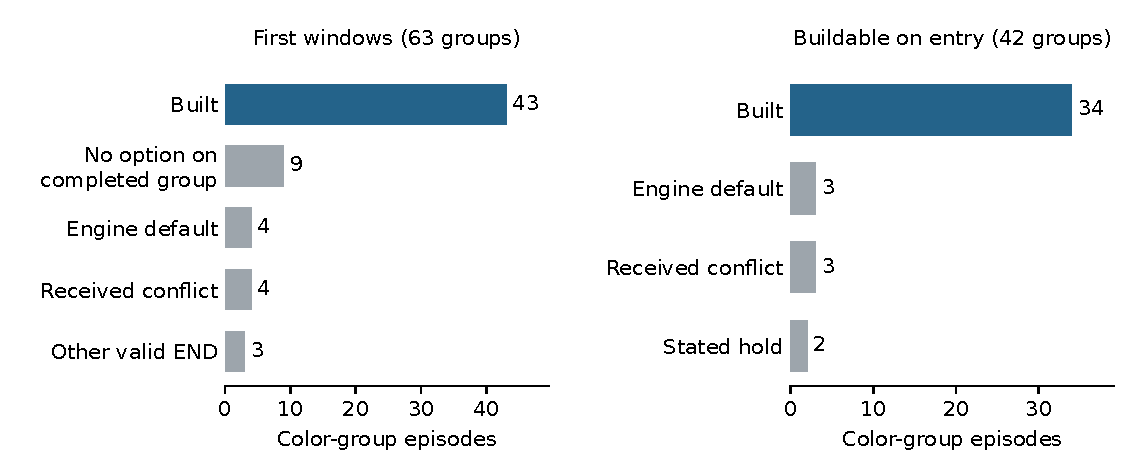
\includegraphics[width=\linewidth]{execution.pdf}
\caption{Development after trade completion. The whole-window population contains 63 groups; the subset buildable on entry contains 42. Availability is measured for the newly completed group. Two G1 no-option windows offer construction on a different group. A received conflict denotes disagreement between content and call, not a validated alternative plan.}
\label{fig:execution}
\end{figure}

Seven of the nine no-option groups receive a mortgaged completing deed. Another, Opus's G20 dark blues, already contains a mortgaged Boardwalk; only Opus's G15 dark blues have no mortgage but insufficient cash for a house. Static budgets at the first post-completion management decision show that two owners can cover redemption and a house with cash alone: Grok has \$602 against \$193 plus \$200 in G14, and \$523 against \$111 plus \$100 in G16. Counting currently mortgageable deeds outside the target group supplies the budget in five more cases. The remaining two fall short of this mortgage-only budget. Bank houses are available in all nine.

The budgets distinguish immediate access from financing choices (Appendix~\ref{app:access}). All four Grok notes explicitly defer redemption or construction to preserve liquidity. In its two G1 windows, the menu also offers an Atlantic house on the already-owned yellow group; Grok declines that investment too. G16 Opus redeems Park Place and ends with \$75 while two other deeds remain mortgageable. Thus a newly completed group can remain undeveloped because its owner preserves cash or collateral elsewhere, even when a static financing budget is sufficient.

Among the forty-two groups buildable on entry, thirty-four receive construction. The eight residuals comprise three defaults, three conflicts and two stated holds. Financing can also precede a conflict: Grok mortgages deeds before its G8, G12 and G13 build-requesting responses end the turn instead. The G8 and G13 content names one-house-per-deed plans consistent with the displayed cash, stock and target keys; the G12 3/2/2 encoding would fail per-entry evenness. G20's content names a mortgage. These plans were not newly executed for this study, but the records distinguish attempted investment from a stated choice to wait.

The broader record contains 663 applied \End{} actions on management menus offering construction somewhere. Sixty-six are defaults and twenty-four are content/call conflicts; in twenty-two of those conflicts the content names construction. Appendix~\ref{app:conditions} retains this accounting separately from the group-level windows.

\subsection{Construction requests, recovery and reserve choices}

All sixty-one defaulted Opus construction purchase multisets execute in the retained historical checks after count-valued entries are split and purchases legally interleaved. Cash, stock and requested purchases are unchanged. The submitted plans remain invalid. Sixty chains have a provider refusal followed by invalid action-only construction; G2 d129 has invalid construction followed by refusal. In both orders the response budget is exhausted and the engine ends management.

Other configurations often recover a rejected construction request. Among uneven-build rejections ending in construction, the original purchase multiset is preserved in 20/25 Sol, 6/18 Gemini and 5/5 Grok decisions. A changed allocation can also be a successful correction. G14 d145--148 realizes an initial eight-house target over several management decisions even though its first correction does not preserve that target. Appendix~\ref{app:validation} gives the full target and default accounting.

Reserve choices are also explicit. At G3 d176, Opus ends with \$204 and its action-only assistant content prefers retaining cash to buying an available \$150 house. At G1 d426, Grok declines another yellow house with \$488, citing its financing needs. These are expressed choices to retain liquidity, distinct from requested builds that the response path does not execute.

\subsection{Realized receipts and a rival's construction budget}

Trade-completed groups receive \$57,378 in rent from completion until loss or game end. The forty-three groups built on in the first window collect \$53,810; the twenty others collect \$3,568, and eleven of those are built on later. Early development and later receipts therefore occur together in this corpus. These are total paid receipts, including undeveloped rent, under differing exposure and survival times. Appendix~\ref{app:economy} gives the per-configuration totals.

Across the 103 game/player/group spending units, construction outlay is \$103,450 and whole-game paid developed rent is \$93,000. Forty receive no developed rent, although some still trigger a creditor elimination. The distinction matters economically: a rent demand can transfer an estate rather than appear as a cash receipt. Salvage, inherited buildings and terminal unpaid debts are accounted for separately in Appendix~\ref{app:economy}.

\TranscriptTitle{g20}{An appeal to withhold a rival's building cash}

In G20, Opus sells Illinois to Grok for \$500, completing reds and leaving Grok \$222. A red house costs \$150. Gemini addresses the table:
\TranscriptQuote{g20-coordination-appeal}
Grok's next note recognizes the appeal:
\TranscriptQuote{g20-recognition-note}
That decision's received call ends management while its content requests a mortgage. After later construction, Grok tries to sell Vermont to Gemini for \$150. Gemini replies:
\TranscriptQuote{g20-concrete-refusal}
\TranscriptFinding{Grok mortgages Vermont for \$50 instead. Opus later makes two cash offers for Grok's property; neither settles. Gemini wins.}
\TranscriptReading{Gemini explicitly asks others to deny a rival construction funds, Grok recognizes the appeal, and Gemini follows through when offered a purchase. Sol had already recorded its own financing objection privately at d95. Opus later offers cash expressly for Grok's house funding, but Grok rejects or counters those bids. The observed coordination is therefore an appeal and its author's follow-through, not a jointly adopted cartel.}
\TranscriptSource{G20 d95--102, d129--130 and d156--160. The appeal is in Grok's d97 request. The quoted note belongs to selected attempt 1 after a malformed first attempt.}
\FloatBarrier

\section{Current-debt finance and creditor inheritance}
\label{sec:finance}

\subsection{Payable debt, genuine insolvency and inaccessible assets}

The sixty eliminations include fifty-six declarations and four automatic terminations. In fifty-six cases, the current debt exceeds the generous own-asset bound in Equation~\ref{eq:bound}: the player's own sales and mortgages cannot pay. Of the remaining four, three have legal payment routes and one is blocked by the implemented liquidation menu despite sufficient nominal assets (Figure~\ref{fig:finance}).

\begin{figure}[H]
\centering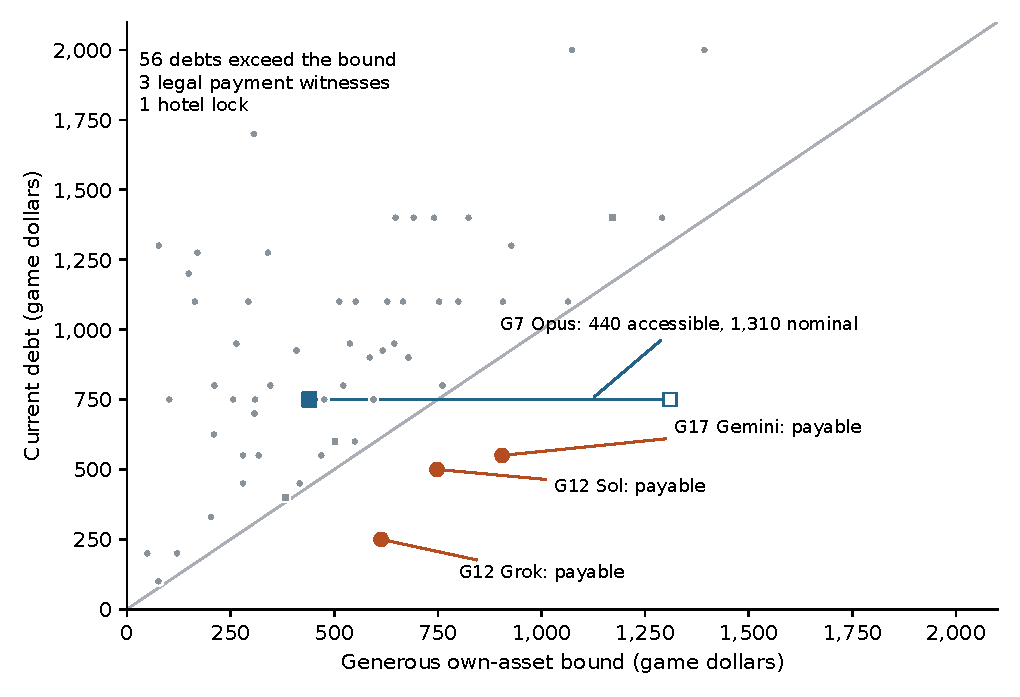
\includegraphics[width=0.9\linewidth]{finance.pdf}
\caption{Debt and the generous own-asset bound at all sixty eliminations. Points above the diagonal exceed the bound. The G7 segment separates nominal resources (1,310) from reachable cash (440) against a debt of 750. Squares mark the four automatic eliminations; G7 has a filled reachable-cash marker and a hollow nominal-bound marker. Payment witnesses concern the current debt.}
\label{fig:finance}
\end{figure}

The payable cases have distinct evidence. Sol's G12 d190 and Gemini's G17 d234 accounts omit collateral unlocked by building sales. Retained witnesses pay debts of \$500 and \$550 and leave \$38 and \$180 respectively. Cash plus immediately mortgageable deeds falls short in both, but that subtotal is not the entire menu, which includes sales. The third case is a same-response conflict, shown below; it can be resolved by house sales alone.

G7 d339 shows why nominal assets and usable finance differ. Opus owes \$750, has \$390 and can mortgage Oriental for \$50. Its pinks have four houses, four houses and a hotel, while the bank has no houses. The sale menu lists only highest-built deeds and offers a hotel sale only when four bank houses can replace it. It therefore offers no sale action, only the Oriental mortgage and bankruptcy. The retained continuation reaches \$440 and automatic bankruptcy despite \$1,310 in nominal resources. This is a menu-level restriction; Appendix~\ref{app:rules} distinguishes it from the separate validator's broader treatment of bundled sales.

The record also shows correct financing and insolvency judgments. At G20 d327--336, Sol combines \$49 cash, \$700 building salvage and \$665 mortgages to pay a \$1,400 debt, leaving \$14. In G16, Gemini declares bankruptcy at the first debt menu with \$288. Its note correctly calculates that \$375 of building salvage and \$730 of mortgages would bring the total to only \$1,393 against a \$2,000 debt. The first is an executed payment sequence; the second is a correct calculation of an unpayable position.

\TranscriptTitle{g12}{A payable debt ends in contradictory execution}

At G12 d249, Grok owes \$250 and has \$43. Its pink group has two, two and three houses. Assistant content requests a Virginia sale:
\TranscriptQuote{g12-sale}
The attached private note concludes:
\TranscriptQuote{g12_d249_private_final}
The sole received tool call instead declares bankruptcy, with this public message:
\TranscriptQuote{g12_d249_public_bankruptcy}
\TranscriptFinding{The engine eliminates Grok without selling houses, transferring its estate to Opus. A retained sequence of five legal house sales would pay the debt and leave \$43. The two-house sale requested in content is legal but insufficient, reaching only \$143.}
\TranscriptReading{The private note initially calls payment impossible, then derives the five-sale route and its correct \$43 remainder, although it miscounts the houses left. The received call nevertheless declares bankruptcy, and its public message supports that action. This separates recognition of a payment route from its execution: the record contains the financing reasoning and an incompatible applied action.}
\TranscriptSource{G12 d249, standard attempt 0. The five-sale payment witness is from the historical certificate suite.}

The disagreement also occurs in the other direction. In seven other Grok records, content names bankruptcy while the received call mortgages a deed in five or sells buildings in two. Those financing actions are not necessarily sufficient to pay; their source records are retained in the archive.

\subsection{Estates redistribute groups while the game continues}

During continuing play, estates complete fifty-two groups, forty-five owned by eventual winners; eighteen of sixty-three trade-completed groups belong to eventual winners. The contrast describes concentration conditional on the same games' outcomes. Across all stable acquisition boundaries there are 209 episodes: sixteen through direct purchase, nine through auction, sixty-three through trade and 121 through inheritance. Sixty-nine inherited completions occur at the final elimination and provide no further management opportunity (Table~\ref{tab:routes}).

\begin{table}[t]
\centering\small
\begin{tabularx}{\linewidth}{@{}lrrY@{}}
\toprule
Completing acquisition & Episodes & Eventual winner & Further play\\
\midrule
Trade & 63 & 18 & All episodes have a management window\\
Direct purchase & 16 & 12 & Before game end\\
Auction & 9 & 2 & Before game end\\
Nonterminal estate & 52 & 45 & Play continues\\
Terminal estate & 69 & 69 & No later management or income\\
\bottomrule
\end{tabularx}
\caption{Completion routes and eventual owner outcomes. Winner status is determined by the same trajectory, so these columns describe concentration rather than an effect on victory. Inherited deeds can also contribute to groups completed later by another route.}
\label{tab:routes}
\end{table}

Trade transfers 207 deeds. Estates transfer 397, including 227 before the final elimination. Eventual winners receive 202 of those 227 nonterminal deeds and are creditors in 35 of forty nonterminal eliminations, compared with 54 of sixty overall. The eventual winner receives the first estate in eighteen games and all three estates in sixteen. In 57 of sixty eliminations, including 38 of forty nonterminal ones, the debt is rent on the creditor's developed color deed. An established rent-producing position can therefore be followed by further asset concentration through inheritance. These counts describe that sequence, not inheritance's separate contribution to victory.

Routes also differ in income and timing. Fifty-one of sixty-three trade-completed groups collect rent, totaling \$57,378 after completion; directly purchased completions collect \$23,070. Estate-completed groups collect \$11,472, with fourteen of fifty-two nonterminal episodes receiving any rent. Later acquisition leaves less exposure, and rent on inherited buildings need not involve new spending. Of fifty-eight winner spending units, thirty-four contain an inherited deed at first own expenditure, while only thirty first become complete through an estate. Four mixed-route units close through a later purchase or trade.

Two winners, Sol in G14 and Gemini in G15, settle no trade. Gemini's G15 orange group completes through a Tennessee purchase and receives its first build on turn 47. It later collects \$3,250 in developed orange rent. Oranges trigger the first two eliminations; inherited browns trigger the last. The green group completes only through the terminal estate. The trajectory connects an early bank purchase to rent income, creditor acquisitions and the final elimination.

\subsection{Negotiating over prospective estates}

The creditor rule gives every player a stake in a distressed opponent's fate. The next exchanges explicitly refer to that stake. They also show why a later trajectory cannot establish the success or sincerity of a prior pitch.

\TranscriptTitle{g13}{An insurance pitch omits an available mortgage}

At G13 turn 107, Grok has \$35, owns yellow and stands nine squares before Short Line, where Sol's four railroads charge \$200. Ventnor remains unmortgaged and is worth \$130 in mortgage cash. Grok offers its mortgaged Pennsylvania to Opus for \$200:
\TranscriptQuote{g13-opening-insurance}
Opus counters at \$130 and records a reason to keep Grok solvent. That account follows Grok's opening appeal; it is not an independently established motive preceding the seller's framing. Grok replies:
\TranscriptQuote{g13-seller-counter}
Its applied note recognizes the Ventnor route and sets a \$165 floor. Returned provider reasoning also states:
\TranscriptQuote{g13-omission-explanation}
Opus accepts:
\TranscriptQuote{g13-acceptance}
\TranscriptFinding{Opus pays \$200 and \$16 mortgage-transfer interest. Seven turns later it buys North Carolina at auction for \$650, completing its greens with the acquired Pennsylvania. In the retained conditional acceptance branch, \$130 plus Grok's \$35 and a later \$130 Ventnor mortgage gives \$295, enough for the threatened rent. Grok does not land on Short Line on its next roll. It later pays \$200 on B\&O at turn 146, leaving \$49, and goes bankrupt on Short Line at turn 150; the yellows pass to Sol.}
\TranscriptReading{Grok frames the sale as insurance against Sol inheriting its estate and expressly describes omitting available collateral in one returned explanation. Opus echoes the estate stakes and pays \$200, but does not affirm the claimed \$130 financing limit. The opening appeal also overstates the landing probability: Short Line is nine squares away, a 4/36 roll, not 5/36. The d252 explanation itself considers accepting \$130 before countering at \$200. The record shows selective disclosure, buyer uptake of the estate framing and a settled price, while leaving the cause of the \$70 difference unidentified. Later bankruptcy follows the actual trajectory; it does not measure survival time purchased by the deal.}
\TranscriptSource{G13 d250--253, d307 and d311; auction purchase event 1911. Grok uses standard responses; Opus uses action-only recovery, with provider explanations rather than applied private notes. The focal recipient requests contain the messages and a garbled history line, alongside correct holdings.}

\TranscriptTitle{g18}{A repeated price is withdrawn after the seller deteriorates}

Opus repeatedly offers \$250 for Sol's mortgaged Pacific, which would complete Opus's greens. After receiving \$750 rent from Sol, it repeats the assurance:
\TranscriptQuote{g18-assurance}
A second \$750 payment then forces Sol to sell orange buildings and mortgage its remaining red deeds, leaving \$49. After larger packages fail, Sol invokes the advertised price:
\TranscriptQuote{g18-invocation}
\TranscriptQuote{g18-withdrawal}
Opus's returned explanation supplies a reason:
\TranscriptQuote{g18-withdrawal-explanation}
\TranscriptFinding{No sale occurs at \$250. Opus redeems Pennsylvania at turn 190 and North Carolina at turn 192, then bids \$150 and \$225 for Pacific at turn 194. Sol asks \$450 and \$350 and later offers it at \$300; none settles. Opus eventually receives Sol's estate and wins. The earlier assurance is present in the requests at invocation and withdrawal.}
\TranscriptReading{The withdrawal changes the terms rather than ending interest in the group. Opus's explanation cites the cost of prolonging a nearly bankrupt rival and of developing greens, yet it redeems its two green deeds and resumes bidding below the withdrawn price. These actions document continued bargaining after the seller's financial deterioration. The standing offer is a public assurance without an engine-enforced commitment; the record identifies no costly action taken in reliance or dishonesty when the original assurance was made.}
\TranscriptSource{G18 d421--461. Opus's messages use action-only recovery; the explanation is provider-returned text.}

\section{Planning across turns and responding to feedback}
\label{sec:temporal}

The temporal sample contains three decisions from each of eighty player-games, selected by a salted hash from an earlier pool of public-message-unflagged records. One LLM-assisted reader examined the complete applied public and private fields, excluding provider explanations. Of the 240 decisions, fifty-nine contain forward-looking own-action statements, thirty-six contain prospective opponent-capacity or outcome statements, and twenty-five refer to correction or feedback, with overlap. Grok accounts for thirty-nine of the fifty-nine own-action records and twenty-two of the thirty-six opponent records. Fifty-three private fields are absent, all for Opus. These counts characterize the selected records rather than estimate a corpus-wide planning rate.

Most statements are contingent or open-ended rather than scoreable commitments. Eight specify buying a named property on landing there. Six never meet a later matching purchase opportunity. One is carried out. The other, Grok's G16 Virginia plan, encounters an affordable purchase menu at d159 with \$371 against a \$160 price. Its note still favors purchase and its public message claims the pink set is closed, but the received call starts an auction. Gemini buys the deed for \$380. This is an observed failure of follow-through with conflicting channels, not an identified change of mind or memory failure.

A positive longer target appears in G9. Sol's turn-29 note plans three houses on each dark-blue deed as funds arrive. Construction and financing over subsequent turns reach that target on turn 60. The sequence demonstrates an expressed target and its later realization; it does not show that retaining the note caused the outcome. The G15 offers likewise respond to an opponent's stated objection, while other notes make checkable deductions about publicly visible cash and collateral. These are concrete forms of opponent attention, rather than calibrated predictions of hidden beliefs.

The complete uneven-build recurrence ledger follows 114 error decisions to 109 later build submissions. Of fifty successors after a decision containing a corrective request with the validator message, nine repeat the error. Of fifty-nine successors without that feedback, fifty-four repeat it; all fifty-nine belong to Opus, whose refusal path consumed the corrective opportunity. The contrast documents repair and recurrence under different response conditions. Because feedback and configuration coincide, it does not identify feedback-caused learning.

\section{Discussion}
\label{sec:discussion}

\subsection{What the participants negotiate}

Participants bargain over positions extending beyond the exchanged deed. They discuss a rival's construction reserves, the value of withholding a completing property and whether funding a distressed seller benefits a third-party creditor. The offer census places those considerations in context: outright refusal is more common when only the offer author completes a group, even within opening and later offers, while counters commonly preserve the exchange and ask for better terms. The transcripts show what that bargaining involves. In G15, a recipient refuses its own completion after the proposer addresses a liquidity objection. In G2, Sol quotes different prices to different buyers, while Opus advertises a lower ceiling than its private contingency permits. These are observable responses to interdependent economic stakes.

The conduct spans successful exchange, refusal, factual correction and changed assurances. G7's bluff settles at the advertised price. G19's recipient corrects a false claim and still accepts the exchange. G13's seller selectively presents its financing options while the buyer discusses the estate at risk. G18's buyer withdraws a repeated price and resumes bidding after the seller deteriorates. Public deception is permitted in this task, so these incidents describe strategic conduct under that contract. Their context shows both what the tactic sought and what happened next, without attributing the resulting price or victory to the tactic alone.

\subsection{From ownership to income and control}

The next question is whether a negotiated position becomes productive. The systems complete similar numbers of groups by trade---seventeen, eighteen, fifteen and thirteen---but build on sixteen, seventeen, seven and three in the first management window. Those early-built groups collect \$53,810 of \$57,378 in post-completion rent. Owners sometimes preserve cash or defer redemption; elsewhere the response path prevents a requested build. Following acquisition into financing and construction thus connects bargaining with the income the position actually produces.

Financial access also determines what can happen at a debt endpoint. Sol's G20 sequence realizes \$1,365 from sales and mortgages to meet a \$1,400 bill, whereas Gemini's G16 calculation correctly recognizes that all available own resources fall short. Across the sixty eliminations, fifty-six debts exceed even the generous asset bound. These endpoints establish the immediate financing position, leaving the quality of earlier spending as a separate question.

Inheritance then extends the economic consequences beyond the eliminated player. Eventual winners receive thirty-five of forty nonterminal estates, and thirty-eight of those forty eliminations follow rent on developed property. A productive group can therefore be followed by acquisition of the debtor's remaining assets. This pathway explains why participants discuss who would inherit a blocker or a complete group. G13's insurance pitch and G18's withdrawn offer make that concern explicit; G15's bank-purchased oranges and subsequent estates show the corresponding sequence in play. Bargaining, development and creditor succession belong in the same account because the assets and incentives carry through all three stages.

\subsection{Scope of the motivating research questions}

Table~\ref{tab:questions} distinguishes direct population descriptions, contextual observations and constructs that remain unmeasured. An unresolved construct is not a negative capability result.

\begingroup\footnotesize
\renewcommand{\arraystretch}{1.09}
\begin{longtable}{@{}L{0.22\linewidth}L{0.36\linewidth}L{0.36\linewidth}@{}}
\caption{The eight motivating questions and three broader questions receive different kinds of evidence. The table is a scope map, not a benchmark scorecard.}\label{tab:questions}\\
\toprule
Question & Evidence in this cohort & Not established\\
\midrule\endfirsthead
\toprule
Question & Evidence in this cohort & Not established\\
\midrule\endhead
\bottomrule\endfoot
1. Strategic reasoning & Offer responses, stated rival consequences, local financing alternatives & Optimal actions, regret or exploitability\\
2. Opponent modeling & Public-capacity deductions and responses to stated objections & Calibrated hidden-belief or preference inference\\
3. Negotiation, cooperation and deception & Complete response census; selected bluffs, omission, correction, withdrawal and coordination appeal & Persuasion effects, fairness, joint surplus, agreement bias or deception prevalence\\
4. Long-horizon planning and memory & Acquisition-to-income trajectories; targets with later opportunities; documented memory conditions & Memory benefit or a general plan-completion rate\\
5. Adaptability and learning & Revisions, successful repairs and repeated errors under observed feedback & Feedback-caused learning or adaptation to unfamiliar opponents\\
6. Economics and risk & Realized flows, construction feasibility and all current-debt endpoints & Ex ante asset values, optimal reserves or risk-adjusted returns\\
7. Collective dynamics & Creditor concentration and a recognized financial-denial appeal & Coalition incidence, stability or a causal coordination effect\\
8. Validity and generalization & Reconstruction under the preserved implementation; explicit response and information conditions & A clean model ranking, corrected-interface performance or external transfer\\
\midrule
A. Strategic talk and action & Cases of realized targets, factual correction and conflicting execution & A general relation between explanation quality and strategic quality\\
B. General versus multi-agent capability & Not evaluated & A capability curve or transfer relationship\\
C. Skill, chance and opponent weakness & Descriptive seed/seat patterns and specific economic pathways & Their causal shares in victory or a counterfactual winner\\
\end{longtable}
\endgroup

Outcome patterns illustrate why the distinction matters. Sol wins one four-rotation block from every seat. In another block, all four configurations win from seat 2, whose player purchases both dark blues by turn 29. In G13--15, seat 1 completes orange through direct purchase on turn 47 under Opus, Sol and Gemini respectively, and wins each game. In the fourth rotation, G16, seat 1 is Grok: it completes orange by trade on turn 116 and loses. Thus seven games share early same-seat purchase paths across different configurations, while four follow Sol across seats. The purchases, subsequent decisions and random events are all part of the observed paths; these patterns do not establish that early dice decided seven outcomes. Across the cohort Sol wins eight games, Gemini seven, Opus three and Grok two. Neither pattern isolates strategic skill or chance, and no independent general-capability axis is measured.
\FloatBarrier

\section{Related work}

\paragraph{Negotiation and economic agency.} NegotiationArena studies bargaining through controlled tactic changes~\cite{bianchi2024negotiationarena}. Recent work distinguishes expressed counterparty modeling from better agreements, including experiments that supply coarse ranked preference information~\cite{cosentino2026counterparty}. MERIT studies feedback for bargaining under specified buyer and seller utilities~\cite{merit2026}. Those designs provide criteria for agreement quality that our multi-player game does not. Our response and cash tables describe the exchanges proposed, while exact counter transitions show how their terms change; neither supplies an optimal-utility reference.

Vending-Bench studies sustained operation of a simulated business~\cite{backlund2025vendingbench}. Its Arena communication study analyzes 2,583 emails over twenty year-long simulations, checks factual claims against simulator records, studies promise follow-through and repeats its pipeline with other judge families~\cite{li2026arena}. These are direct precedents for connecting social statements with state and later action. Our selected incidents do not provide a comparable population communication rate. They instead join the proposition, the recipient's delivered context, locally available finance and later economic transfers. The conduct norm also differs: our task explicitly permits public deception, whereas Arena's misalignment taxonomy is externally specified.

\paragraph{Games and configured-system evaluation.} AgentMonopoly examines model families, sizes and personas through Monopoly actions and language~\cite{wu2026agentmonopoly}. Its paper's prompt encourages bluffing while prohibiting public messages contradicting the action~\cite[\S4, App.~A.2]{wu2026agentmonopoly}. The repository implementation inspected at commit \texttt{2434f427} accepts or rejects single offers and eliminates at negative cash without the debt-liquidation step studied here; it also transfers buildings intact to a player-creditor~\cite{agentmonopoly2026repo}. The counteroffers and liquidation sequences in our corpus extend the economic trajectory available for study under these different rules.

FinBoardBench evaluates financial decisions across board games, including Monopoly counteroffers~\cite[\S3.2]{hu2026finboardbench}. Its main decision phase permits up to five execution failures before a recorded system-forced fallback~\cite[App.~E]{hu2026finboardbench}. Its Monopoly bankruptcy treatment sells buildings to the bank~\cite[App.~C.3]{hu2026finboardbench}, so its return summaries concern a different accounting setting from receipts on inherited development here. DECE studies complete model-and-execution configurations across ten Eurogames and runs matched execution-framework comparisons~\cite{zhang2026dece}. HAL likewise motivates evaluating complete agent systems~\cite{kapoor2026hal}. Our observational study follows those configurations through bargaining, construction and creditor transfers.

\paragraph{Interpreting agent behavior.} Work on explanation faithfulness distinguishes recorded reasons from internal computation~\cite{turpin2023unfaithful,lanham2023faithfulness}; MASK distinguishes honesty from factual accuracy~\cite{ren2025mask}. Agent-evaluation reliability and measurement-focused auditing likewise motivate explicit units and evidence requirements~\cite{hardy2026reliability,yang2026measurement}. We combine that discipline with complete economic trajectories: the state establishes the stakes, the delivered messages establish exposure, and later actions establish the observed outcome.

\section{Limitations}

The cohort has five seeds, four cyclic rotations per seed and a fixed opponent roster. States and responses are dependent, opponent identities are visible, and response conditions are confounded with configuration. Opus's refusal recovery changes its prompt, retry opportunities and memory; Grok has unresolved disagreements between response channels; some delivered histories misattribute past trades. These conditions are reported before the results and attached to affected analyses. They preclude intrinsic model rankings and claims about corrected interfaces or unfamiliar opponents.

The ruleset and observational design limit economic conclusions. Intact creditor inheritance and restricted building stock shape the available strategies. The bargaining categories differ in assets, prices and stages, cash thresholds are exploratory, and eventual-winner splits condition on the same trajectories. We measure realized flows and local financing possibilities, without identifying optimal prices, causal persuasion or the separate contributions of skill and chance. Appendix~\ref{app:rules} gives the implementation and historical-witness scope.

Semantic evidence is retrospective and LLM-assisted. Research assistants selected incidents and developed coding categories after inspecting the records; Sol and Opus assistants share model identifiers with two evaluated participants under different tasks and settings. Two partly unblinded reason readings are not independent human validation. Six of the eight main incidents involve Grok, whose channels are unusually observable, so the selection cannot estimate or rank conduct prevalence. Exact quotes and delivered-context checks make the interpretations inspectable. Full research roles and artifact provenance are recorded in Appendix~\ref{app:reproducibility}.

\section{Conclusion}

The twenty games show agents negotiating over rival development, financing productive assets and anticipating who will inherit when a player fails. Recipients sometimes refuse their own group completion because of the rival position it enables; counters often preserve the exchange while seeking better terms. Completed groups generate income through subsequent financing and construction, and developed-property rent precedes most creditor acquisitions. Eight contextual incidents show bluffing, correction, selective disclosure, financial-denial appeals and withdrawal alongside those economic trajectories. Together, the population accounts and transcripts explain how stated strategies become bargains, income and control of assets in these four configured systems.

\begingroup\small
\bibliographystyle{plainnat}\bibliography{references,supplemental}
\endgroup
\clearpage\appendix
\newcommand{\CohortRows}{%
1 & 1 & 1 & 216 & Gemini & 3 \\
2 & 1 & 2 & 102 & Gemini & 2 \\
3 & 1 & 3 & 283 & Gemini & 1 \\
4 & 1 & 4 & 166 & Grok & 1 \\
5 & 2 & 1 & 170 & Sol & 2 \\
6 & 2 & 2 & 126 & Sol & 1 \\
7 & 2 & 3 & 150 & Sol & 4 \\
8 & 2 & 4 & 139 & Sol & 3 \\
9 & 3 & 1 & 88 & Sol & 2 \\
10 & 3 & 2 & 75 & Gemini & 2 \\
11 & 3 & 3 & 145 & Grok & 2 \\
12 & 3 & 4 & 166 & Opus & 2 \\
13 & 4 & 1 & 185 & Opus & 1 \\
14 & 4 & 2 & 110 & Sol & 1 \\
15 & 4 & 3 & 114 & Gemini & 1 \\
16 & 4 & 4 & 386 & Sol & 3 \\
17 & 5 & 1 & 118 & Sol & 2 \\
18 & 5 & 2 & 197 & Opus & 4 \\
19 & 5 & 3 & 175 & Gemini & 1 \\
20 & 5 & 4 & 115 & Gemini & 4 \\
}

\newcommand{\ResponseRows}{%
Sol & Author only & 83 & 2 & 50 & 31 \\
Sol & Recipient only & 30 & 6 & 21 & 3 \\
Sol & Both & 8 & 1 & 6 & 1 \\
Sol & Neither & 114 & 21 & 63 & 30 \\
Gemini & Author only & 76 & 4 & 9 & 63 \\
Gemini & Recipient only & 31 & 6 & 10 & 15 \\
Gemini & Both & 34 & 6 & 12 & 16 \\
Gemini & Neither & 100 & 10 & 5 & 85 \\
Opus & Author only & 52 & 7 & 42 & 3 \\
Opus & Recipient only & 42 & 5 & 31 & 6 \\
Opus & Both & 11 & 2 & 7 & 2 \\
Opus & Neither & 83 & 15 & 60 & 8 \\
Grok & Author only & 78 & 6 & 10 & 62 \\
Grok & Recipient only & 37 & 7 & 16 & 14 \\
Grok & Both & 28 & 1 & 10 & 17 \\
Grok & Neither & 111 & 14 & 41 & 56 \\
}

\newcommand{\EliminationRows}{%
1 & 315 & Opus & declared & 118 & 550 & 318 & Below debt \\
1 & 454 & Sol & declared & 41 & 200 & 121 & Below debt \\
1 & 485 & Grok & declared & 30 & 1,275 & 170 & Below debt \\
2 & 215 & Opus & declared & 117 & 1,300 & 927 & Below debt \\
2 & 239 & Sol & declared & 77 & 1,300 & 77 & Below debt \\
2 & 278 & Grok & declared & 203 & 330 & 203 & Below debt \\
3 & 240 & Opus & declared & 77 & 1,100 & 552 & Below debt \\
3 & 426 & Sol & declared & 414 & 2,000 & 1,074 & Below debt \\
3 & 601 & Grok & declared & 147 & 925 & 617 & Below debt \\
4 & 244 & Sol & declared & 49 & 550 & 469 & Below debt \\
4 & 279 & Gemini & declared & 86 & 750 & 256 & Below debt \\
4 & 348 & Opus & declared & 210 & 625 & 210 & Below debt \\
5 & 226 & Grok & declared & 306 & 900 & 586 & Below debt \\
5 & 272 & Gemini & declared & 149 & 1,200 & 149 & Below debt \\
5 & 309 & Opus & declared & 84 & 1,100 & 799 & Below debt \\
6 & 154 & Grok & declared & 235 & 750 & 595 & Below debt \\
6 & 220 & Opus & declared & 32 & 750 & 102 & Below debt \\
6 & 232 & Gemini & declared & 91 & 800 & 211 & Below debt \\
7 & 287 & Grok & declared & 531 & 1,400 & 1,291 & Below debt \\
7 & 304 & Gemini & declared & 11 & 1,400 & 741 & Below debt \\
7 & 339 & Opus & automatic & 390 & 750 & 1,310 & Hotel lock \\
8 & 271 & Gemini & declared & 133 & 700 & 308 & Below debt \\
8 & 280 & Grok & declared & 86 & 1,100 & 666 & Below debt \\
8 & 287 & Opus & declared & 9 & 750 & 309 & Below debt \\
9 & 183 & Gemini & declared & 383 & 1,100 & 913 & Below debt \\
9 & 197 & Grok & automatic & 1,081 & 1,400 & 1,171 & Below debt \\
9 & 220 & Opus & declared & 54 & 1,400 & 824 & Below debt \\
10 & 188 & Sol & declared & 232 & 1,400 & 692 & Below debt \\
10 & 193 & Opus & declared & 28 & 1,400 & 648 & Below debt \\
10 & 198 & Grok & declared & 509 & 600 & 509 & Below debt \\
11 & 225 & Gemini & declared & 349 & 1,100 & 1,064 & Below debt \\
11 & 228 & Opus & declared & 306 & 1,700 & 306 & Below debt \\
11 & 325 & Sol & declared & 293 & 1,100 & 753 & Below debt \\
12 & 190 & Sol & declared & 53 & 500 & 748 & Payable \\
12 & 249 & Grok & declared & 43 & 250 & 613 & Payable \\
12 & 343 & Gemini & declared & 24 & 1,100 & 164 & Below debt \\
13 & 213 & Gemini & declared & 228 & 950 & 538 & Below debt \\
13 & 311 & Grok & declared & 49 & 200 & 49 & Below debt \\
13 & 355 & Sol & declared & 16 & 100 & 76 & Below debt \\
14 & 209 & Opus & declared & 246 & 800 & 346 & Below debt \\
14 & 222 & Gemini & declared & 162 & 800 & 522 & Below debt \\
14 & 234 & Grok & declared & 522 & 1,100 & 907 & Below debt \\
15 & 203 & Grok & declared & 241 & 800 & 761 & Below debt \\
15 & 221 & Opus & declared & 170 & 950 & 645 & Below debt \\
15 & 276 & Sol & declared & 180 & 450 & 280 & Below debt \\
16 & 431 & Opus & declared & 280 & 550 & 280 & Below debt \\
16 & 447 & Grok & declared & 93 & 1,100 & 628 & Below debt \\
16 & 602 & Gemini & declared & 288 & 2,000 & 1,393 & Below debt \\
17 & 234 & Gemini & declared & 0 & 550 & 905 & Payable \\
17 & 267 & Opus & declared & 63 & 1,100 & 293 & Below debt \\
17 & 398 & Grok & declared & 366 & 750 & 476 & Below debt \\
18 & 344 & Gemini & automatic & 302 & 400 & 382 & Below debt \\
18 & 360 & Grok & declared & 64 & 950 & 264 & Below debt \\
18 & 463 & Sol & declared & 149 & 900 & 679 & Below debt \\
19 & 225 & Grok & automatic & 382 & 600 & 502 & Below debt \\
19 & 284 & Opus & declared & 34 & 925 & 409 & Below debt \\
19 & 322 & Sol & declared & 242 & 1,100 & 512 & Below debt \\
20 & 274 & Grok & declared & 77 & 450 & 417 & Below debt \\
20 & 310 & Opus & declared & 225 & 600 & 550 & Below debt \\
20 & 354 & Sol & declared & 130 & 1,275 & 340 & Below debt \\
}

\newcommand{\AccessRows}{%
1 & 298 & Grok & Orange & 229 & 200 & 100 & 205 & 134\\
1 & 314 & Grok & Dark Blue & 369 & 221 & 200 & 130 & 78\\
8 & 268 & Opus & Brown & 7 & 33 & 50 & 300 & 224\\
12 & 236 & Opus & Light Blue & 31 & 66 & 50 & 460 & 375\\
14 & 207 & Grok & Dark Blue & 602 & 193 & 200 & 185 & 394\\
15 & 57 & Opus & Dark Blue & 158 & 0 & 200 & 0 & -42\\
16 & 234 & Grok & Orange & 523 & 111 & 100 & 215 & 527\\
16 & 248 & Opus & Dark Blue & 268 & 193 & 200 & 200 & 75\\
20 & 297 & Opus & Dark Blue & 125 & 221 & 200 & 150 & -146\\
}

\newcommand{\PriceRows}{%
All & 1.312 (131) & 1.389 (176) & 1.625 (87) & 1.083 (113)\\
Unmortgaged & 1.536 (88) & 1.500 (143) & 2.321 (37) & 1.818 (59)\\
Opening & 1.400 (70) & 1.364 (103) & 1.100 (41) & 0.793 (55)\\
Later & 1.250 (61) & 1.429 (73) & 2.113 (46) & 1.912 (58)\\
}

\section{Cohort and response populations}
\label{app:cohort}

The five seeds, in block order, are 751774554, 2506298840, 2573692901, 3648314310 and 2766649504. Seats and rotations are one-based. The cyclic design covers four of 24 possible seat orders, not every order. Table~\ref{tab:cohort} preserves the twenty-game mapping used by the incident identifiers.

\begin{table}[htbp]
\centering\small
\begin{tabular}{rrrrlr}
\toprule
Game & Block & Rotation & Turns & Winner & Seat\\
\midrule
\CohortRows
\bottomrule
\end{tabular}
\caption{The complete cohort. Winner totals are descriptions of these dependent trajectories, not estimates of an intrinsic ranking.}
\label{tab:cohort}
\end{table}

\begin{table}[htbp]
\centering\small
\begin{tabular}{llrrrr}
\toprule
Recipient & Newly completes & Offers & Accept & Counter & Reject\\
\midrule
\ResponseRows
\bottomrule
\end{tabular}
\caption{All acceptance-legal responses by recipient and completion category. This table exposes the Opus exception to the pooled one-sided acceptance and rejection patterns.}
\label{tab:response_cells}
\end{table}

The 526 threads include 414 with an earlier thread between the same pair in the same game. Among opening offers, 524 permit acceptance and receive 32 accepts, 137 counters and 355 rejects. The 394 later offers receive 81 accepts, 256 counters and 57 rejects. The complete response population adds two acceptance-ineligible openings, one countered and one rejected. Initiation propensity uses own turns with a legal proposal opportunity: Sol proposes on 83/834, Gemini 16/766, Opus 160/660 and Grok 106/676. Multiple threads can begin in one turn, so these are not the thread totals in the main text.

The counter join follows every one of 394 counter responses to the next offer in its thread, checks actor reversal and compares exact completed groups and noncash bundles. The 92/111 retained-completion result concerns the same original author's group; retaining its requested deeds selects those same ninety-two records. Of the eighty-eight counters leaving only that party completing, eighty-five improve negotiated cash for the counterer. The median improvement across all eighty-eight is \$125, and the direction agrees after transfer-interest accounting. Seventy-nine are pure cash repricings of unchanged deeds and cards; nine change noncash terms too. Sol and Opus author ninety-two of the 111 author-only counters and eighty of the 110 non-completing counters.

The pooled author-only versus recipient-only rejection ordering holds in all five seed blocks and seventeen of nineteen games containing both categories. Recipient-level comparisons pool thread position. Separating opening and later offers for Sol, Gemini and Grok gives the same rejection ordering in five of six cells and the same acceptance ordering in three of six, with one tie and two reversals. These cuts expose composition within the cohort; they are not independent replications.

The exploratory cash cuts use cash immediately before the offer, not net worth or maximum accessible finance. Among cash settlements with sellers below thresholds of \$50, \$100, \$150 and \$200, respectively, 14/20, 21/30, 22/36 and 24/40 complete the paying party's group. The denominator conditions on a low-cash seller and a settlement. It differs from the main-text 21/48, which conditions on all payer-completing cash settlements. Opus is the cash receiver in sixteen of the thirty below-\$100 settlements. These composition differences preclude a causal distress interpretation.

\subsection{Cash direction and board-price comparisons}
\label{app:prices}

The completing side receives at least one deed in every one of the 429 one-sided completion offers. It pays net cash in 373: authors pay in 238 author-only offers and recipients in 135 recipient-only offers. Cash also flows toward the net deed seller in 309 of 313 non-completing offers with unequal deed counts. The two denominators differ, but both exhibit ordinary buyer-to-seller payment. Median signed cash toward the recipient is \$200 for author-only completion, $-350$ for recipient-only, $-100$ for both and \$100 for neither. These are transaction terms, not evidence that a recipient is offered free money or a completion premium.

Table~\ref{tab:prices} restricts the comparison to acceptance-legal offers exchanging cash for deeds, with no countervailing deed, cash or jail-card transfer. The ratio divides negotiated cash by the sum of the received deeds' board list prices. Bids have the current author offering cash; asks have the author offering deeds. Unmortgaged means no mortgage-transfer interest is due on the proposed exchange. Ratios are computed before rounding; the table prints three decimals and the number of offers.

\begin{table}[htbp]
\centering\small
\begin{tabular}{@{}lrrrr@{}}
\toprule
& \multicolumn{2}{c}{Buyer bids} & \multicolumn{2}{c}{Seller asks}\\
\cmidrule(lr){2-3}\cmidrule(lr){4-5}
Subset & Author completes & Neither & Recipient completes & Neither\\
\midrule
\PriceRows
\bottomrule
\end{tabular}
\caption{Median cash divided by board list price, with offer counts in parentheses. These are overlapping descriptive cuts, not matched valuation comparisons.}
\label{tab:prices}
\end{table}

The buyer-side ordering reverses between the pooled or later-offer cuts and the unmortgaged or opening-offer cuts. The ask-side ordering remains higher for recipient completion in the displayed cuts. Both parties choose what to offer; property mix, negotiated rights, state and negotiation stage remain uncontrolled. Board price supplies a fixed arithmetic denominator, not fair value, strategic value or a causal completion premium. These exploratory cuts are not used to score pricing skill.

\section{Economic units and the complete elimination ledger}
\label{app:economy}

\begin{table}[htbp]
\centering\small
\begin{tabularx}{\linewidth}{@{}L{0.25\linewidth}Y@{}}
\toprule
Unit & Definition and boundary\\
\midrule
Attempt & One saved provider response, including refused or invalid responses.\\
Decision & One engine menu resolved into one applied action, possibly through several attempts.\\
Offer & One current proposal or counter awaiting the other party's response.\\
Completion episode & Ownership of every deed in a color group, from completion until loss or game end.\\
First management window & The owner's first actual management turn after completion, including all its management decisions.\\
Spending unit & One game/player/color triple with positive own construction expenditure.\\
Elimination & One declared or automatic bankruptcy.\\
\bottomrule
\end{tabularx}
\caption{Units are preserved separately. In particular, an attempt, an offer, a spending unit and an elimination are not interchangeable observations.}
\end{table}

Paid rent totals \$121,154 over 905 payments. Trade moves \$28,425 through 107 directed cash transfers and 207 deeds. Estates move \$11,830 and 397 deeds; before the final elimination, the amounts are \$7,843 and 227 deeds. Eventual winners receive \$7,148 and 202 of those nonterminal transfers. No cash and deed quantities are summed into one flow statistic. Rent on trade-completed groups until loss or game end is \$20,818 for Sol, \$26,070 for Gemini, \$5,930 for Opus and \$4,560 for Grok. This ordering differs from the win totals and is not a return or skill ranking.

Of twenty terminal estates, nineteen go to the eventual winner and G13's goes to the bank. The 54 winner-creditor eliminations therefore comprise thirty-five nonterminal and nineteen terminal cases. Terminal creditor identity is not automatically the winner in this implementation.

The 103 spending units have \$103,450 construction outlay, \$93,000 whole-game developed rent and \$92,550 developed rent after first own expenditure. The counts of forty zero-developed-rent units and twenty-six also lacking a creditor elimination concern units. Fifty-seven developed-color rent elimination triggers concern events. Winner spending includes fifty-eight units, thirty-four with inherited deeds at first own spending and thirty first completed through an estate. The four mixed routes are G3 p1 brown, G6 p1 light blue, G12 p2 light blue and G14 p1 green. This distinction prevents possession of an inherited deed from being equated with estate completion.

\subsection{Financing budgets without an option on the completed group}
\label{app:access}

Table~\ref{tab:access} reads the first post-completion management prompt for each of the nine groups without a recorded build option on that group during the window. Every target group is complete, has no buildings, and has bank houses available. G1 d298 and d314 offer construction on Atlantic, outside the target groups. Redemption $R$ uses the preserved floating-point ceiling. Outside mortgages $M$ include only deeds listed as mortgageable in that prompt and exclude the target group. The last column is cash plus $M$, less $R$ and one house's cost. A nonnegative budget is not an executed multistep witness; a negative budget rules out only this specified financing budget, not every possible liquidation or trade.

\begin{table}[htbp]
\centering\small
\begin{tabular}{@{}rrllrrrrr@{}}
\toprule
G & d & Owner & Group & Cash & $R$ & House & $M$ & Remainder\\
\midrule
\AccessRows
\bottomrule
\end{tabular}
\caption{Static budgets at nine recorded management decisions, in game dollars. Two cover redemption and a house with existing cash, and five additional budgets do so using current outside-group mortgage options.}
\label{tab:access}
\end{table}

The four Grok notes explicitly defer redemption or construction for liquidity reasons. Their quoted redemption amounts---\$198 for the G1 orange deeds, \$220 for Boardwalk and \$110 for New York---are correct under the exact ten-percent rule. The implementation instead charges \$200, \$221 and \$111 because of floating-point ceilings (Appendix~\ref{app:rules}); the table uses those implemented charges. Management prompts do not supply redemption prices. Mortgaging an outside deed can also disable another complete group, so a budget is not a recommendation. In G16 Opus's dark-blue window, the actual Park Place redemption leaves \$75, while Reading and B\&O remain mortgageable for \$100 each.

Table~\ref{tab:all_eliminations} records all sixty current-debt classifications. The three payable cases have sufficient witnesses, not maximal liquidation claims. Other retained witnesses for G12 Sol and G17 Gemini leave \$8 and \$155 because they mortgage different collateral. G12 Grok's witness uses five house sales and no mortgages. G7's only financing continuation is the Oriental mortgage, followed by automatic bankruptcy.

\begin{longtable}{rrllrrrl}
\caption{Every elimination. All monetary values are game dollars. ``Below debt'' means the generous bound is below the debt; ``Payable'' means a legal payment witness exists.}\label{tab:all_eliminations}\\
\toprule
G & d & Debtor & Termination & Cash & Debt & Bound & Classification\\
\midrule\endfirsthead
\toprule
G & d & Debtor & Termination & Cash & Debt & Bound & Classification\\
\midrule\endhead
\bottomrule\endfoot
\EliminationRows
\end{longtable}

\section{Implementation and certificate scope}
\label{app:rules}

The preserved ruleset is \texttt{audit\_corrected\_v2}. Free Parking pays nothing, income and luxury taxes are \$200 and \$100, and jail permits up to three doubles attempts before a forced fine. A player remaining jailed has no management window that turn. Model-facing state includes opponents' configured names.

Transfer interest and redemption both use floating-point ceilings. Multiplying mortgage principal by 0.1 agrees with the exact board-principal transfer charge. Multiplying by 1.1 for redemption exceeds the exact mathematical ceiling by one dollar for principals \$50, \$90, \$100, \$110 and \$200. A \$100 mortgage therefore costs \$111 to redeem in this implementation. Historical alternatives use that actual charge. The present paper does not establish whether each overcharge changed an affordability boundary.

Build validation checks evenness after each plan entry. Sale validation can accept a bundled operation from final evenness and net stock. An atomic one-building-at-a-time search can therefore miss a legal bundled sale. The corrected checker refuses negative graph certificates in states offering building sales. Its retained negative graph result is the G7 mortgage-only state, whose menu offers no sale action. Source inspection indicates that the separate sale-plan validator would accept a \$650 group-clearing bundle if a sale were offered; that observation is not a new executed witness. G7's lock is a restriction of the authoritative legal menu, not a proof that every mathematical liquidation of its buildings is impossible.

\label{app:validation}
The portable historical suite contains sixty elimination cases and sixty-six construction defaults. Fifty-six eliminations use the arithmetic upper bound, three use payment witnesses and one uses the restricted search. The defaults contain seventy well-formed targets, one malformed target and sixty-one attempts with no parseable target. Of the seventy well-formed targets, sixty-three execute after reordering and seven exceed cash. Sixty-three of the sixty-six decisions contain at least one reachable target. Fifty-five defaults are concentrated in G5 and G13, including thirty-nine in G13. These are complete declared populations, not 126 independent mechanisms.

The portable package preserves original action streams, settings, event digests, a fixed case manifest and unchanged engine/board copies. It reproduces its supplied cases. Population completeness, original attempt extraction and semantic interpretation require the separately retained ledgers and raw records. A successful reproduction cannot supply those missing claims by itself.

The broader reconstruction checks match 10,235 economic snapshots and all 113 accepted settlements, including \$431 mortgage-transfer interest across thirty settlements. Rebuilt initial memory matches all 6,989 prompts. Jail-card transfers require transaction and bankruptcy context rather than dedicated transfer events, though reconstructed card holdings match 27,956 player observations. This is a limitation of the event vocabulary, not a reason to infer an unrecorded change.

The retained certificate replay compares every complete event after JSON serialization with sorted keys, compact separators and ASCII escaping. It does not drop event fields or normalize away identifiers in this comparison. Raw-file whitespace and key order therefore need not be byte-identical, while the decoded event values must agree. Other state-only replay modes have different scopes and are not the basis of the 50,918-event equality reported here. Engine determinism, correspondence to intended Monopoly rules, and validity of a behavioral interpretation remain separate claims.

Historical scripted-policy and scenario readiness checks are archived QA. They are not strategic comparators for the four-player cohort and are not pooled into any reported capability result.

\subsection{Recorded response and information conditions}
\label{app:conditions}

Opus has 1,605 refusal-affected decisions but 1,604 first-attempt refusal recoveries: G2 d129 adds a refusal on the second attempt. The configured policy names \texttt{anthropic/claude-opus-4.8} as a third-stage fallback, but it is never invoked; all 1,696 decision records return Opus 5.5, and no decision exceeds two attempts. At 1,394 later memory windows, no model-authored private note is carried forward: 1,108 have an empty field and 286 carry fallback text. The jump in first-attempt refusals coincides with the source-commit boundary. The inspected diff changes campaign concurrency, UI, documentation and tests, with no engine, prompt or model-client change; it identifies no cause of the provider behavior.

Among Grok's 1,663 decisions, the retained parser identifies 1,068 initial content action names: 1,035 from parsed JSON, twenty-three from malformed content with a name, and ten from flat action forms. There are 139 disagreements with the received call name, fifteen with equal parsed argument objects and five with equal literal argument substrings. The saved requests are non-streamed and the responses are single received JSON bodies. The records therefore locate the disagreement in the received response, without identifying how the provider or upstream service produced it.

The historical trade formatter reverses attribution for forty-four accepted settlements, also misstates twenty-six rejected threads, and produces 232 self-partner references. Affected summaries occur in 2,054 delivered prompts. Current holdings remain correct, and all 920 current trade-response menus were reconciled separately. Of 6,882 applied nonempty public messages, 149 never enter the public timeline and thirteen enter it without a later recipient request carrying them. Transcript delivery checks use the actual recipient request.

Structured board parameters vary by phase. All 547 purchase prompts supply the landed deed's price, house cost, rents and group; all 854 auction prompts supply its group. Management, trade, jail and liquidation prompts identify deeds by space keys without those board-price fields, and none of 4,081 management prompts states redemption costs. Calculations can draw on prior observations, messages or remembered board values, but the current structured menu is not itself a complete price or rent reference.

Of 663 applied ends on menus offering construction somewhere, sixty-six are engine defaults and twenty-four disagree with the action named in content. Twenty-two of those twenty-four content actions request a build, one a mortgage and one a proposal. The remaining 573 are not thereby classified as deliberate reserve choices. Opus accounts for sixty-one defaults among its 104 such ends. In the separate construction-recovery population, exact within-decision multiset recovery occurs in 20/25 Sol, 6/18 Gemini, 5/5 Grok and 0/61 Opus cases; broader recovery definitions retain different denominators and are preserved in the audit files.

\section{Contextual controls and transcript provenance}
\label{app:transcripts}

Three controls remain available beyond the eight main incidents. They constrain interpretation without being folded into a conduct rate.

\subsection{G11: a false completion claim corrected before a true one is refused}

In G11's two-player phase, Sol offers Virginia for Grok's Pennsylvania while claiming Virginia completes the pink group. It does not, because Sol also holds St. Charles. Grok replies:
\TranscriptQuote{fx-g11-reject}
Sol's note repeats its false premise, so the available records do not establish that the original statement was knowingly false. Sol corrects the offer:
\TranscriptQuote{fx-g11-concede}
\TranscriptQuote{fx-g11-reject-again}
The second offer genuinely completes Grok's pinks, but Grok still cites Sol's green completion. This is correction followed by a rival-sensitive refusal, contrasting with G19's correction followed by acceptance. The stronger two-player position and different terms prevent a controlled comparison. All four public messages at G11 d255--258 are verified in the counterparties' next requests.

\subsection{G3: a false stock obstacle with a prior hold}

At G3 d363, one house remains in the bank and Gemini can potentially add a Park Place house. Grok says:
\TranscriptQuote{G3-2}
Its own note contains a contrary route:
\TranscriptQuote{G3-3}
Gemini's next note gives a reserve and income reason:
\TranscriptQuote{G3-5}
The retained conditional route mortgages two deeds and buys the one house, establishing that the claimed stock obstacle is false for that route. Gemini had already held before the statement. Delivered misinformation followed by another hold therefore does not establish reliance, while the conflicting source channels prevent a simple unified-intent attribution.

\subsection{G20: a private fragment reaches public chat}

At G20 d1, a private-note fragment is already embedded in the received public-message argument:
\TranscriptQuote{g20-received-and-applied-public}
The engine emits it, and Gemini subsequently records recognition:
\TranscriptQuote{g20-recipient-recognition}
Assistant content requests an empty public message. The disclosure and recognition are observed. Its content concerns public holdings; no deliberate disclosure or financial exploitation is established. Decision d1 is the second decision of the game.

\subsection{Selection, fields and exact excerpts}

The eight main incidents preserve distinct mechanisms rather than maximizing a severity score. Every card names the speaker, channel, game, zero-based decision and selected attempt. Public messages are emitted with applied actions; private notes are the attached \texttt{private\_thought} fields; returned provider explanations and assistant content are separate response fields. Bracketed ellipses mark omitted spans. Errors in quotes, including the G2 nine-house claim, remain unchanged.

Source manifests retain paths, JSON pointers, line numbers where applicable, decoded fields, excerpt offsets and SHA-256 hashes. Quote checks reload original fields. Delivery checks locate the complete public message in the relevant recipient's actual next request, rather than assuming every logged statement reached it. They establish exposure only. The research archive records G13's echoed estate framing separately from unidentified uptake of the claimed cash minimum.

\section{Reproducibility and research roles}
\label{app:reproducibility}

Code and the twenty saved games are public at \url{https://github.com/KushagraBharti/MonopolyBench}. Checkpoint \texttt{a10419d239ff75f9e75a77d1634261a6ca24148c} preserves the preceding manuscript and research record. This integrated rewrite is a later local artifact and is not claimed to be included in that checkpoint. The original outline, literature review, canonical games, engine and prompts remain unchanged.

The research-assistant team comprises GPT-6 Astra, GPT-6.1 Sol, Claude Opus 5.5 and Claude Fable instances under human direction. Earlier work used Fable 5.1; this rewrite used fresh Fable 5.2. Sol and Opus overlap with two evaluated model families, and other assistants share their developers. Each wrote an entire independent manuscript before reading the other drafts and performing whole-paper review. This procedure broadens scrutiny but does not create independent human labels or an inter-rater validity standard.

The final manuscript combines retained mechanical audits with existing-record checks. Re-tabulations reproduce offer cells, counter transitions, construction populations and estate routes. All displayed quote spans are checked against their original fields, with focal recipient delivery checked separately. The original engine-executed witnesses, full replays, memory reconstruction and semantic coding remain inherited analyses. Document builds and rendered-page checks establish presentation and internal correspondence.

The package includes native LaTeX, figure-generation scripts, copied source ledgers, source manifests, build instructions and review records. The independent drafts and disagreements remain archived. The evidence map records the status of each claim and the limits of every verification layer.

\end{document}
